% !TeX encoding = UTF-8
% !TeX program = pdflatex
% !TeX spellcheck = en_US

\documentclass[LaM,binding=0.6cm]{sapthesis}

\usepackage{microtype}

\usepackage[inline]{enumitem}

\usepackage{hyperref}
\hypersetup{pdftitle={DTA-Tracker: a colourful approach to understanding split-personality malware},pdfauthor={Riccardo Chiaretti}}

\usepackage{curve2e}
\definecolor{gray}{gray}{0.4}
\newcommand{\bs}{\textbackslash}

\usepackage{listings}
\usepackage{amssymb}
\usepackage{xcolor}
\usepackage{caption}
\usepackage{parcolumns}

\newcommand{\source}[1]{\caption*{Source: {#1}} }
 
\definecolor{codegreen}{rgb}{0,0.5,0}
\definecolor{codegray}{rgb}{0.55, 0.57, 0.67}
\definecolor{codepurple}{rgb}{0.58,0,0.82}
\definecolor{backcolour}{rgb}{0.91, 1.0, 1.0}
%\definecolor{backcolour}{rgb}{0.74, 0.83, 0.9}
\definecolor{darkblue}{rgb}{0.0, 0.0, 0.55}

\lstdefinestyle{codesnippets}{
    backgroundcolor=\color{backcolour},   
    commentstyle=\color{codegreen},
    keywordstyle=\color{darkblue},
    numberstyle=\tiny\color{codegray},
    stringstyle=\color{codepurple},
    basicstyle=\ttfamily\footnotesize,
    breakatwhitespace=false,         
    breaklines=true,                 
    captionpos=b,                    
    keepspaces=true,                 
    numbers=left,                    
    numbersep=5pt,                  
    showspaces=false,                
    showstringspaces=false,
    showtabs=false,                  
    tabsize=2
}

\lstset{style=codesnippets}

% Commands for the titlepage
\title{DTA-Tracker: a colourful approach to understanding split-personality malware}
\author{Riccardo Chiaretti}
\IDnumber{1661390}
\course{Ingegneria Informatica - Engineering in Computer Science}
\courseorganizer{Facolt\`{a} di Ingegneria dell'Informazione, Informatica e Statistica}
%\course[override]{Master of Science in Engineering in Computer Science}
%\courseorganizer{Faculty of Information Engineering, Informatics, and Statistics}
\AcademicYear{2018/2019}
\copyyear{2020}
\advisor{Dr. Daniele Cono D'Elia}
\authoremail{riccardochiaretti7@gmail.com}

\examdate{20 January 2020}
\examiner{Prof. Nome Cognome}
\examiner{Prof. Nome Cognome}
\examiner{Dr. Nome Cognome}
\versiondate{\today}

\begin{document}

\frontmatter
\maketitle

\dedication{Dedicated to\\ Donald Knuth}

\begin{abstract}
Malware is the abbreviation for malicious software and encompasses all software designed to infiltrate and harm any computer system without the owner consent. Malicious software is one of the most dangerous threats in today world and being able to detect and prevent them is a real challenge. The ability of security professionals to design automatic analysis systems capable of characterising malware behaviours, collides with the cunning of attackers who are always looking for new ways to escape from automatic countermeasures. It is a constant push and pull between developing effective tools for extracting malicious software profiles and split-personality malware which employ an array of anti-analysis measures.\\
Malicious samples which manage to circumvent automatic countermeasures, require manual intervention of a malware analyst. Although it is essential to dismantle new techniques employed by malware authors, manually dissecting a binary is a lengthy process. Identifying before the dissection, which program slices characterise its behaviours, would surely speed-up the whole process. Leveraging the dynamic binary instrumentation technology and adopting the technique of taint analysis, we propose a tool for profiling the interaction between the executable and data it manipulates. Through the possibility of choosing which data to track and the design of a completely new schema, it allows to identify where in the program these data were introduced as well as which program slices accessed them. 
\end{abstract}

\begin{acknowledgments}
ciao
\end{acknowledgments}

\tableofcontents

\mainmatter

\chapter{Introduction}
Over the years, there have been great strides in the world of technology. Amazing devices like smartphones, tablets and computers allow us to have information within easy reach. In a very short period of time, these devices have become so much part of our lives that we now find it impossible to live without. The Internet has established itself as a global medium for the interconnection of people, companies and even appliances with the evolution of Internet-of-Things. At the beginning of $2019$ there were $5.114$ billion unique mobile users and $4.39$ billion internet users in the world\footnote{https://datareportal.com/reports/digital-2019-global-digital-overview.}.\\
Although these new technologies made our life much easier, there exist people who take advantage of them in ways that are not appropriate. The issue becomes increasingly difficult to solve due to the growing number of devices connected to the Internet. \textit{Cybercrime} can be defined as the illegal action where an information system (e.g., mobile device, computer) is a target or a tool\cite{dashora2011cyber}. Information systems are targets of cybercrime in cases of unauthorized accesses, physical damage to systems or also theft of sensitive data. Conversely, information systems serve as tools in activities like email spoofing and financial crimes. The reason behind these attacks is money: in $2018$ the average cost of a data-breach for a U.S. company was $\$7.91$ billions\footnote{https://www.symantec.com/definitions/why-is-cyber-security-important.}. Furthermore, cybercrime costs will exceed $\$2$ trillion by the end of $2019$ and is expected to more than double in $2020$.\\

There are several types of malicious software through which an attacker can achieve his purpose including worms, trojan viruses nad spyware. The concept of malicious software actually, is not something new\cite{Historyo87:online}. Even though the first information systems were not targeted by malicious programs, it does not mean at all that they were invulnerable rather, people were just not aware of the possibility to exploit computer systems. Indeed, according to \cite{Whendidt95:online}, the first malicious threat\footnote{In the field of computer security, a threat refers to any entity which has the potential to harm computers, computer systems, network infrastructures and many other systems. What is defined to be a threat strictly depends on the target information system but, often categorized as threats are: vulnerabilities, people who can infiltrate a system and malicious software.} goes back to $1949$. In particular, the first mathematical definition of a computer virus, was introduced in $1986$ by the computer scientist Fred Choen\cite{cohen1987computer}.\\
However, as technology evolved, malware authors were also able to improve their software: from simple and harmless programs that were able to move across networks\footnote{https://corewar.co.uk/creeper.htm.} or replicate themselves\footnote{https://pandorafms.com/blog/creeper-and-reaper/.} we are now in the era of ransomware, fileless malware\cite{alzurigrowth} 
and advanced persistent threats\cite{virvilis2013big}.\\

Security professionals employ great efforts in designing systems that can disarm malicious software and provide safety to end-users. However, the effectiveness of security products is at odds with the ability of malware writers to devise new mechanism that bypass security countermeasures. Signature-based systems and several automatic analysis systems may be ineffective against these malware category. The ever increasing malware complexity, most of the time, requires the intervention of analysts able to dissect them understanding the underlying logic and behaviour. Manual dissection of executables is time-consuming and it is often unnecessary to inspect each single instruction rather, only on some portions are worth to be analysed. Tracing the interaction between the executable and data, can lighten the analyst work by highlighting where to focus his attention. In this direction, through dynamic taint analysis, it is possible to track data flow in a program by tagging information of interest to understand which program slices involve operations on that data. Nevertheless, providing fine-grained information without incurring in the risk of data overload, results in a careful choice of how to identify tainted data, what introduced them in the execution as well as who actually accessed them. Finally, collected data should also be organized in a scheme that emphasizes the relationships between the parties.
%Despite there are a number of researches based on taint analysis, they all ...
%Information flow tracking is a computer science branch which studying techniques to track the way data flows throughout the program.
%The majority of information flow tracking tools are used to enforce integrity and confidentiality polices on sensitive data. Thus,  without providing fine-grained information

\section{Contributions}
In order to lighten the job of a malware analyst, helping him in the task of binary dissection for understanding its behaviour, this thesis proposes a completely new approach for modelling the interaction between the executable and the data it manipulates. Leveraging the taint analysis technique and Pin DBI framework, we propose DTA-Tracker, a program analysis tool designed on top of BluePill and able to:
\begin{itemize}
\item Taint the output data of several APIs and system calls providing calling context information to help understanding where, in the executable, tainted data is introduced;
\item Accurately identify all memory chunks coloured as a result of data movement operations;
\item Detect where in the program, tainted memory is used as operand in both data transferring and comparison instructions;
\item Organize collected data into a scheme that, as far as we know, was never applied to this end, namely, the producer-consumer graph.
\end{itemize}  

\section{Outline}
The thesis starts by providing the reader with some background knowledge on the main topics related to malware analysis including a discussion about different categories of malware, why is important to set-up a safe analysis environment and challenges that rise in doing so (\autoref{ch:chapter1}). Afterwards, it presents the concepts of information flow, taint analysis and dynamic binary instrumentation  together with tools and libraries through which it is possible to put these techniques into practice (\autoref{ch:chapter2}). Without a thorough discussion of the approach, the reader would not be able to understand design and implementation choices employed in DTA-Tracker (\autoref{ch:dta-tracker}). Ultimately, after discussing few use-cases where our tool may be helpful, we provide some ideas for future developments (\autoref{ch:futureworks}).

\chapter{Background}
\label{ch:chapter1}
What today we know as \textit{malware}, it is nothing but a term coined from the two words \textit{malicious} and \textit{software}. Even though the term malware and malicious software are syntactically different, their meaning remains exactly the same. We adopt the concept of malware as a generic word to denote any malicious program, created by a cybercriminal, to cause harm to a legitimate system.\\

Even before the spread of the internet, malicious software were infecting personal computers by modifying or overwriting boot sectors. Thus, they were just targeting boot sectors or files and were spread through floppy disks. Starting from the $90$s, when the internet became accessible to more people and computer network infrastructures started to expand, distributing malware became easier and the number of viruses out there increased. Specifically, computer programs like Microsoft Office started to be always more adopted, leading malware authors to create viruses tailored to these widespread technology. Given the increased adoption of emails for communication, especially among businesses, virus propagation was not more manual rather became network-oriented.\\
As time goes on during the $21^{st}$ century, the introduction of new technologies and standards brought to benefits both for the increasingly number of offered services but also for their ease of use. Nonetheless, on the computer security point of view, the establishment of new technologies brought information systems to become more and more complex, increasing their attack surface\footnote{In information security, the attack surface is identified as the set of virtual and physical points where an attacker can infiltrate into a computer system\cite{AttackSu36:online}.}. The subsequent invention of exploit kits, allowed the attacker to perform automated attacks exploiting different vulnerabilities present on several websites. Attacks automation brought a situation where plenty of websites were infected leading to the increase of virus distribution.\\
If from one side malware authors were able to adopt several techniques for spreading malwares, at the same time they were capable to reach their goal using different malware categories. 

\section{Malware in the Wild}
\label{sec:malwareinthewild}
The number of different malwares which have been invented, is countless. The same holds for the numerous different techniques employed by a malware author to infect the system and exfiltrate data from it. Despite several countermeasures are already adopted against malicious software, malware authors are always able to propose new hacks to bypass already existing security systems. This back-and-forth between cybersecurity experts and cybercriminals, increases the difficulties faced by security professionals who continuously update anti-malware measures which, otherwise, would not be able to properly avoid these threats.\\
Even though a malicious software can leverage several techniques, here are the main categories that most malware fall into:
\begin{itemize}
\item \textit{Backdoor}. It is a general category to identify malicious code allowing the attacker to have access on a computer. Backdoors usually serve to remotely execute commands on the infected system;
\item \textit{Downloader}. It is often executed when the attacker gains access to a system and its only purpose is to download and install additional malicious software;
\item \textit{Launcher}. Its purpose is to launch malicious programs. To reach the stealthiest behaviour, it usually adopts unconventional mechanisms to launch malicious software;
\item \textit{Information-stealing malware.} This is the category of malware which infects the victim to collect sensitive information (e.g., keyloggers) that is later sent to the attacker;
\item \textit{Rootkit.} It is especially useful to hide the presence of other malicious software. Indeed, rootkits usually come together with backdoors to gain access to a system while concealing its presence;
\item \textit{Worm.} Also known as \textit{virus}, a worm is capable of copying itself and infect additional systems.
\end{itemize}
\begin{figure}[h!]
\centering
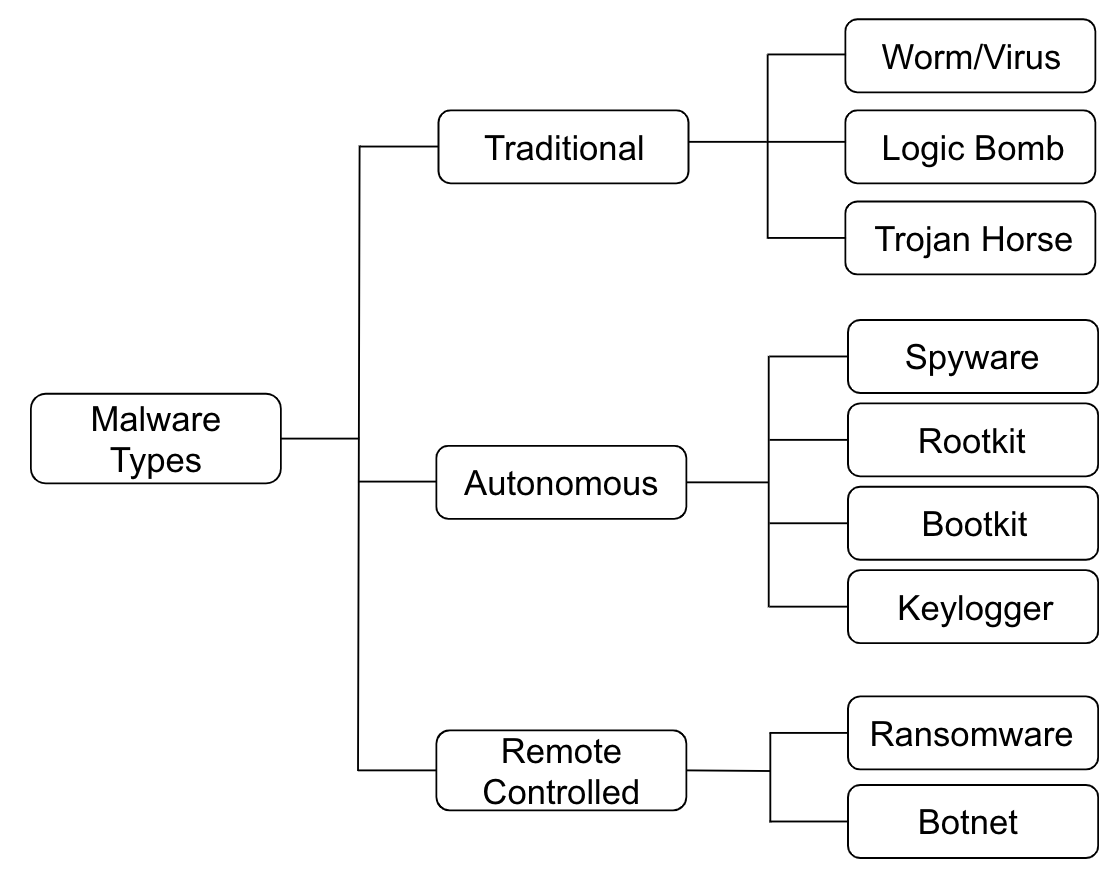
\includegraphics[scale=.5]{images/background1}
\caption{One of several approaches to group malicious software.}
\end{figure}
Although these groups may seem unrelated to each other, malwares often span multiple categories. For example, a sample can have a keylogger which collects passwords while a worm component sends spam messages.

\newpage
\section{Analysing Malwares}
The constant growth of malicious software employed to disrupt information systems, given rise to a new discipline called \textit{malware analysis}. This discipline consists in dissecting malicious software to have a better understanding of its behaviour, how it is be possible to identify it and provide countermeasures\cite{sikorski2012practical}. The figure responsible to carry out the analysis of malwares is called \textit{malware analyst}. The goal of a malware analyst typically consists in identifying the malware executable, determine its behaviour by also recognizing the infected files and endpoints and usually provide information either on how to respond to the attack or how to limit the damage.\\
Once the analysis procedure ends, it is possible to produce an identifier which sums-up some of the main malware features. In the literature, these identifiers are called \textit{signatures} and are usually the final result of automatic malware analysis programs. Specifically, there exist two categories:
\begin{itemize}
\item \textit{Network-based signatures} can be used to detect the presence of malicious code by monitoring the network traffic. Some examples of network signatures can be: a precise pattern in the IP packet denoting a buffer overflow attack or also specific SYN packets\footnote{A SYN is a packet sent by the client to ask a TCP-enabled server to open a new connection.} causing DoS attacks\cite{fuchsberger2005intrusion};
\item \textit{Host-based signatures} identify specific operations performed by the malware on the victim machine (e.g., creation and modification of particular files). Therefore, they are used to detect the presence of malicious code on a computer system.
\end{itemize}
These signatures are usually kept inside a large database and used by Intrusion Detection Systems (IDS), Intrusion Prevention Systems (IPS) or also anti-virus programs to detect or prevent the execution of malicious software. 
\begin{figure}[h!]
\centering
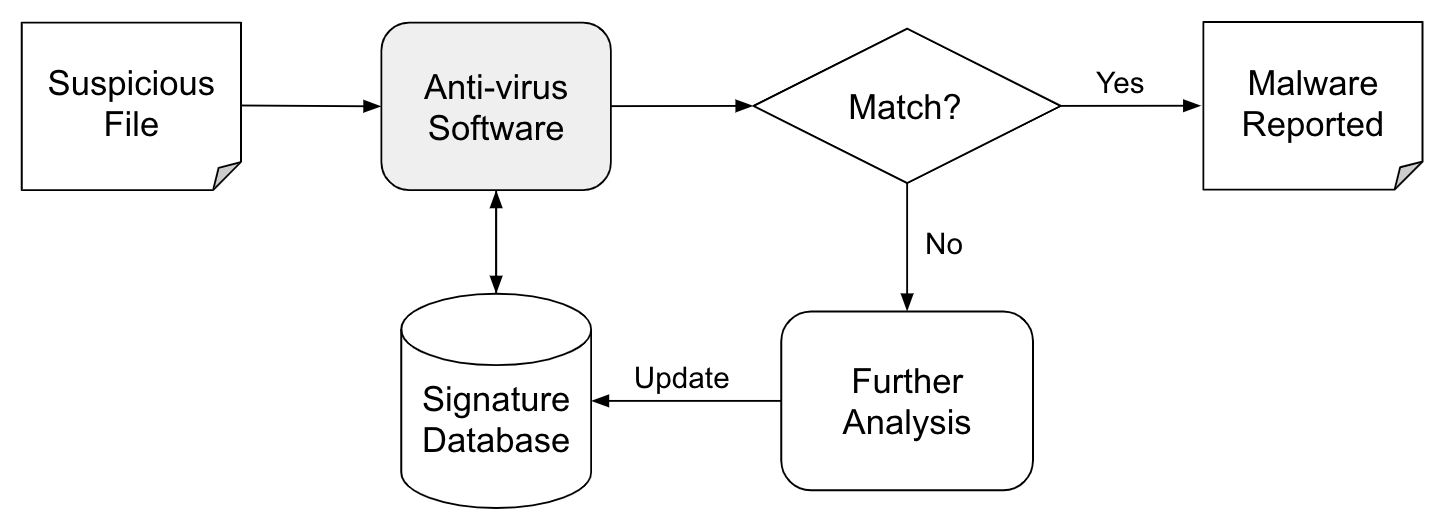
\includegraphics[scale=.5]{images/background2}
\caption{High-level architecture of signature-based anti-virus programs.}
\end{figure}
\newpage
However, today's malware authors use different obfuscation techniques to conceal distinguishing figures of a malware and for this reason, anti-virus programs must adopt more 
sophisticated technology.\\

Independently from how the final result is used, the goal of malware analysis remains always the same: determine the purpose and functionalities of a malware. Nevertheless, there is no straightforward way to carry out the dissection of a malware. Indeed, each malware analyst, has its own preferred tools and techniques which allow him to stand out in his job.

\subsection{Static and Dynamic Analysis}
It is clear that in order to start analysing a malware, we need actually a sample which, most of the times, is not available in a human-readable format (i.e., source code) but only in the form of a binary file.\\ 
Despite the fact that there exist several tools and techniques to carry out the analysis of a malware, the two fundamental approaches to malware analysis are: static and dynamic analysis: 
\begin{itemize}
\item The base concept underlying static analysis, consists in extracting information from the binary without actually executing it. This is the safest way of analysing the malware, as no running code cannot infect any machine. Depending on the level of the technique, the analysis can be divided into basic or advanced.
\begin{itemize}
\item In its most basic form, statically analysing a program does not involve viewing any instruction rather, it uses external tools to infer something about the malware. Computing the hash value of the malware sample, falls into a basic form of static analysis. This can be helpful when used together with services offered by websites like VirusTotal\footnote{https://www.virustotal.com/gui/home/upload.} which provide a set of report from engines which marked the file as malicious. Another useful technique falling into this category, is searching into the executable for hard-coded strings (using tools like pestudio\footnote{https://www.winitor.com/.}) like IP addresses, URLs or even names of imported library functions. If this last step did not produce useful information, it is possible to use PEiD\footnote{https://www.aldeid.com/wiki/PEiD.} to detect if the binary is packed and, in some cases, to know the adopted algorithm. Basic static analysis tools are easy to use and not time-consuming, which is the reason why they are given a chance before resorting to further techniques. However, they can give very limited information and miss important behaviours;
\item Advanced static analysis is also known as code analysis because the binary is dissected to study each single component. Usually, code analysis consists in reverse-engineering the malware by loading the executable into a disassembler (e.g, IDA\footnote{https://www.hex-rays.com/products/ida/.}) to study program instructions. Given that assembly instructions are executed by the CPU, the advanced static analysis objective is understanding what the program does. Although it can be very informative, reverse engineering requires the knowledge of several OS concepts as well as understanding assembler code.
\end{itemize}
\item Dynamic analysis techniques examine the malware while it is running. Often static analysis reaches a dead-end due to the presence of techniques like obfuscation and packing. For this reason, the analyst can resort to executing the malware to have a more in-depth understanding of its behaviour. Just like the static approach, also dynamic analysis techniques can be categorized as basic and advanced.
\begin{itemize}
\item Basic dynamic analysis do not require any complete programming knowledge so, can be used to have an high-level understanding of malware behaviour. Diffing is one of the techniques falling into this category and consist in comparing the system state before and after malware execution (regshot\footnote{http://www.winpenpack.com/main/download.php?view.1170} is a tool which makes possible to take a snapshot and later compare it with another one). Other techniques include monitoring API calls or also collecting system events (e.g., file creation, registry modification and more). Still, most of these techniques are not very effective and sometimes produce a disproportionate amount of false positives (just think to system event caused by all the services running in a Windows host);
\item Advanced dynamic analysis focuses on malware internals rather than externally observable behaviours. This is possible by loading the binary into a debugger to examine the internal state of registers and memory locations. However, since debugging is time-consuming, it is often recommended to try all the previously described approaches and resort to advanced dynamic only as last chance.
\end{itemize}
\end{itemize}

\begin{figure}[h!]
\centering
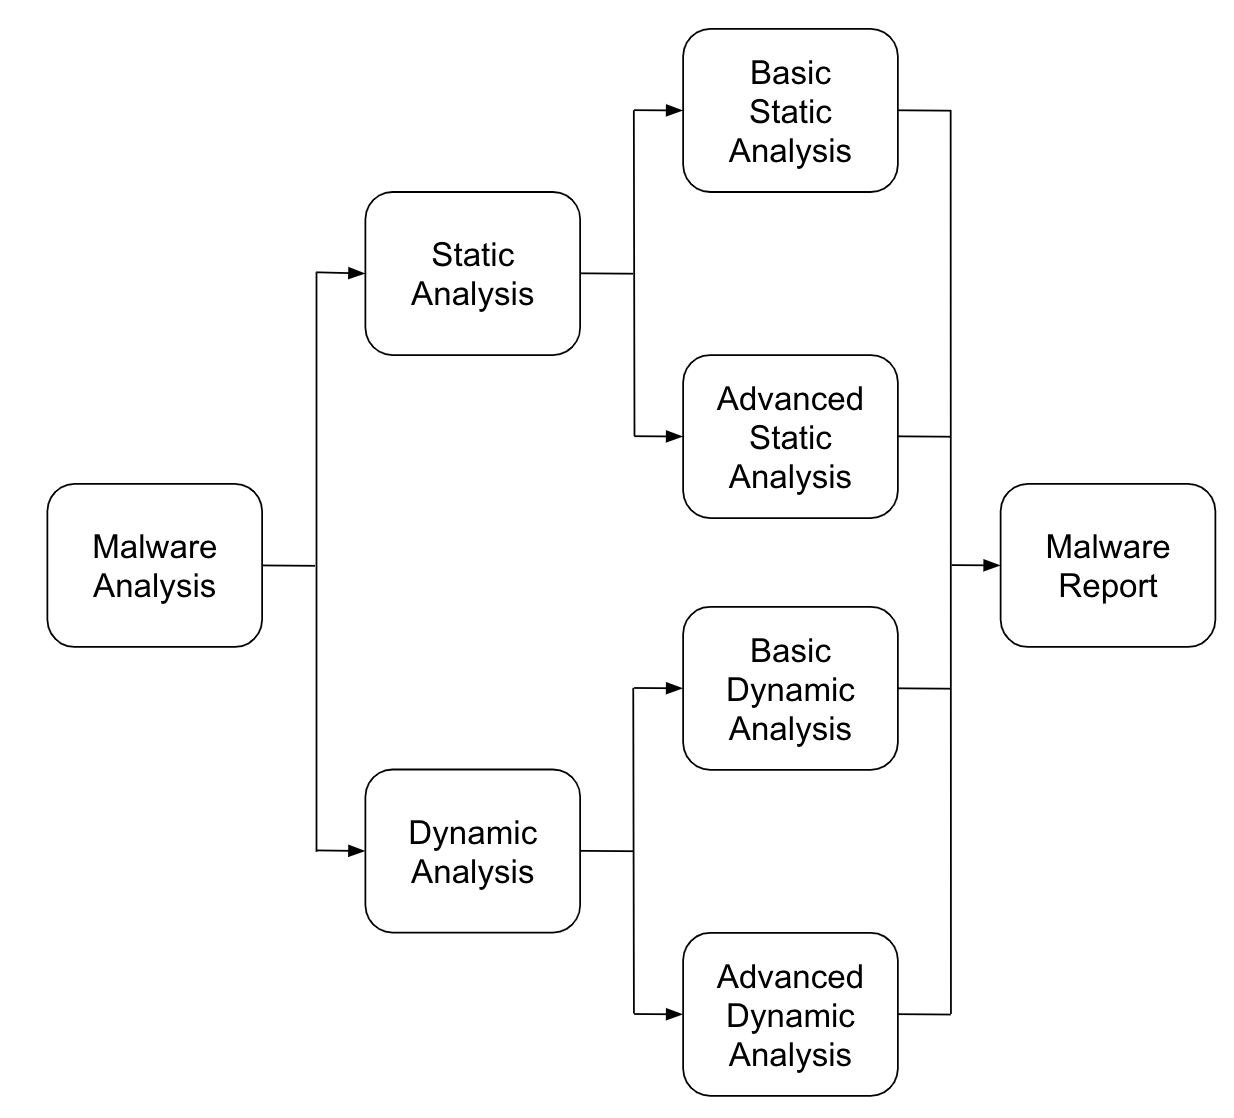
\includegraphics[scale=.5]{images/background3}
\caption{Graphical representation of the fundamental approaches to malware analysis.}
\end{figure}

\newpage
Static analysis is usually one of the first step to get an high-level understanding of what the malware does. Although it is useful, the second step consists in confirming these findings through dynamic analysis. Usually, this is exactly what a malware analyst does when facing a packed malware. Malware writers often decide to obfuscate their malicious software to make it more difficult for analysts to detect and analyse it. Packing manages to reach obfuscation by compressing or encrypting (part of) the malware and using a stub\footnote{When talking about packed software, a stub refers to the module implementing the decryption or decompression routine.} for decryption only when it is executed. For this reason, at first some basic static analysis tool is used to detect whether the malware is packed or not and then, through advanced dynamic analysis techniques, the malware can be unpacked.\\
Therefore, a malware analysis session is not either static or dynamic rather, it consists of a combination of static and analysis techniques. Moreover, especially when dissecting the sample inside a debugger, the analyst must adopt a set of expedients to avoid the infection or limit the damage caused by the malware.

\subsection{Analysis Environment}
\label{subsec:analysisenvironment}
If from one side each analyst uses his own tools and techniques to dissect a malware, from the other side it is fundamental to have a safe environment where to analyse. Since malware are created specifically to harm information systems, if dynamic analysis is performed on common machines (e.g, computer office), it can easily spread through the network and quickly infect other systems. This is why safe environment play an essential role, because they allow the analyst to examine the malware without exposing any machine to unwanted and unnecessary risks.\\
There is not any specific rule to create an analysis environment rather, there exist several combination of tools and techniques which can make it safe. Despite that, analysis environments can be grouped into two different categories:
\begin{enumerate}
\item \textit{Virtualised systems}. They are built upon a virtualisation layer which abstracts hardware resources of a machine. Thanks to hardware abstraction, multiple virtual environments can be built upon a single physical machine: in this scenario the operating system in the physical machine is called \textit{host OS} while the one in the virtual machine is the \textit{guest OS}. One of the several benefits of carrying out the analysis on a virtual machine, is the possibility to quickly restore the system to a previous state. Indeed, it is not rare that a malware modifies settings or critical files leaving the machine in an inconsistent state. Although virtual environments are widely adopted, they do not offer a great transparency and are very resource consuming. To have a boost on resource-consumption, performances and transparency, depending on the purpose, it is possible to design environments that are not fully virtualised but which rely on one or few level of virtualisation;
\item \textit{Bare-metal systems}. These kind of configurations do not use any kind of virtualisation rather, the malware is executed and monitored in a OS running on real hardware\cite{kirat2011barebox}. Bare-metal systems offer the highest transparency thanks to the lack of any virtualisation layer but, at the same time, suffer from other disadvantages. Most of the solutions for system restoring, necessary when the state is inconsistent due to malware execution, require the whole system to reboot. Dynamically analysing a malware is already a time-consuming task and risks getting worse due to external inconveniences.
\end{enumerate}
Choosing the right environment is not an easy task and depends also on the malware under analysis. Indeed, different kind of malware may require different analysis strategies which, in turn, can be fully exploited only on specific analysis systems.
\begin{figure}[h!]
\centering
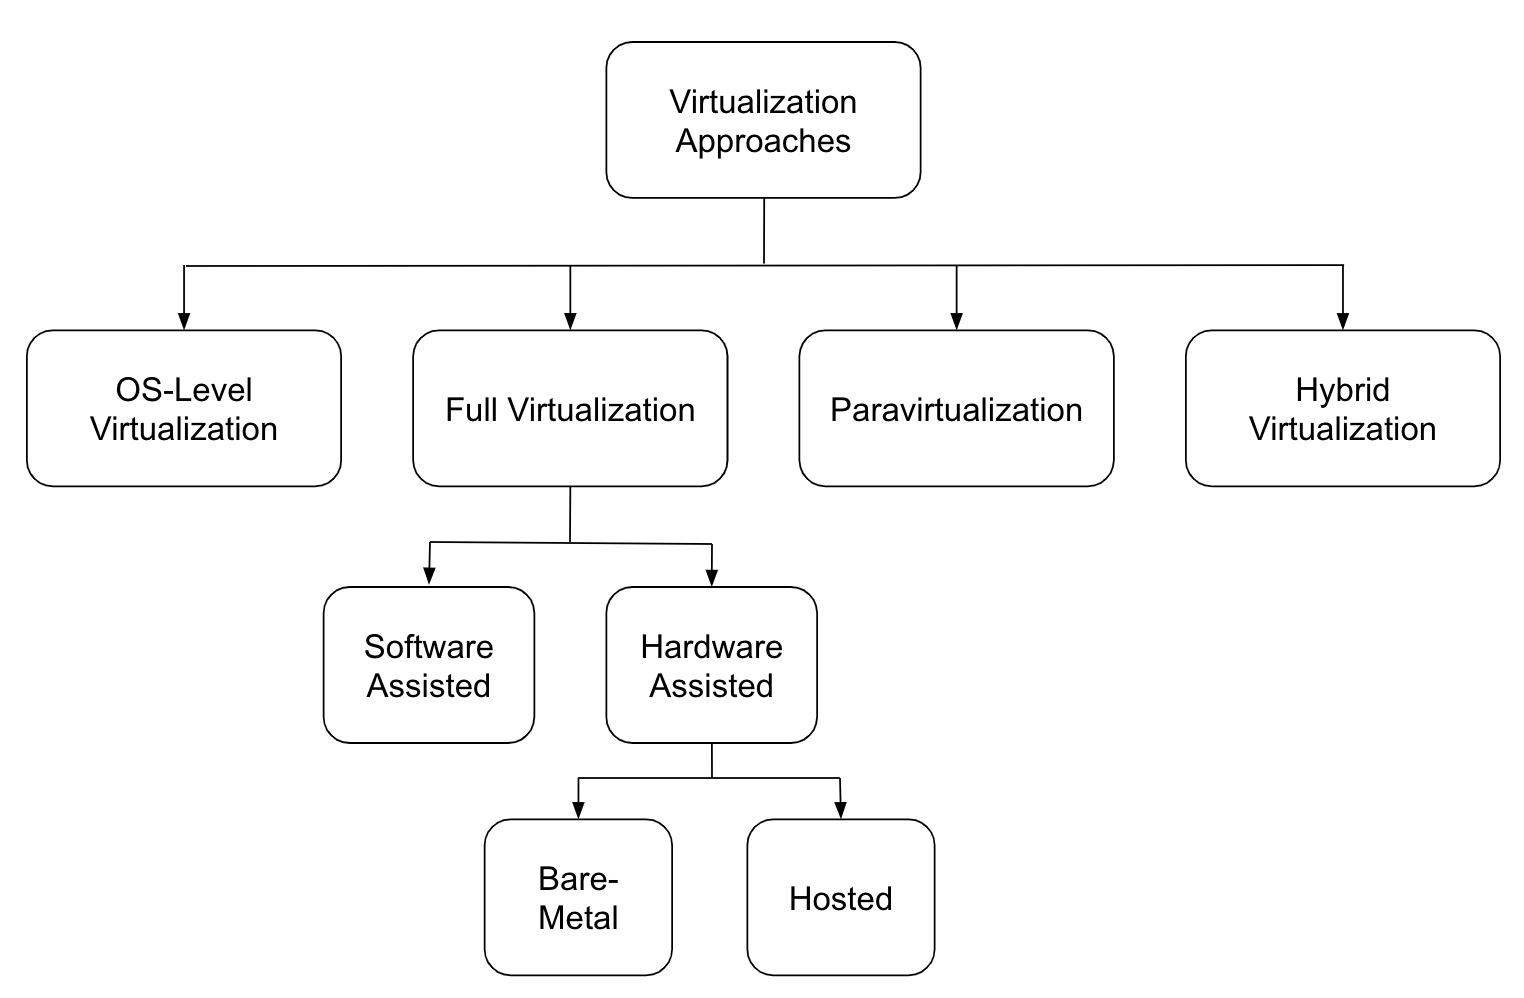
\includegraphics[scale=.5]{images/background4}
\caption{Possible virtualisation categories. The VirtualBox VM can provide software assisted virtualisation, when the underlying host does not enable hardware-assisted virtualisation but it can also act as hosted hypervisor.}
\end{figure}
\newpage
\subsection{Evasive Malware Challenges}
\label{subsec:evasivemalware}
In order to make analysis environments safe, analysts use tool and techniques which isolate the malware as much as possible thus, reducing the harm caused to the system. Virtualised environments are, in this context, the best choice because they avoid that changes on the guest OS can fall back to the host OS. On the other hand, there is not much to do for bare-metal systems where the malware can directly infect the host operating system. Although it may seem that these latter systems are more disadvantageous than virtualised ones, they are the most transparent.\\
The property of an analysis system to be indistinguishable from any non-analysis system, is referred to as \textit{transparency}\cite{bulazel2017survey}. While bare-metal analysis systems can reach a very high transparency level, it would be infeasible due to performance and design reasons, to build a transparent virtual machine\cite{garfinkel2007compatibility}.\\

One category of malwares in addition to those listed in \autoref{sec:malwareinthewild}, is that of \textit{evasive malwares}. Specifically, belong to this group all malicious software whose behaviour is affected by the transparency level of analysis environments. Often, it is considered to be an orthogonal category because evasive techniques are usually added to the malware keeping, at the same time, its original malicious purpose. Evasive techniques installed by the malware author into the software, allow to hinder the malware analyst job making the whole process more time-consuming.\\
Depending on which feature they focus on, evasion techniques\footnote{Here, we refer to evasion techniques which aim to avoid dynamic analysis. A more in-depth description of evasive behaviours against static analysis techniques, can be found at \cite{moser2007limits}.} can be grouped into the following categories:
\begin{itemize}
\item \textit{Environmental artifacts}. The most common evasive behaviours are based on fingerprinting the underlying environment. When an OS like Windows is installed into a virtual machine like Oracle VirtualBox, the latter will add and modify some guest OS settings in order to work properly. This include the creation of specific files or registry keys which include virtual machine identifiers (e.g., the string \texttt{VirtualBox}) in their names. Beyond files and registry keys, other artifacts include the number of running processes, the name of external devices (e.g., disk name) or even the username\cite{lindorfer2011detecting};
\item \textit{Timing attacks}. In the virtualisation context, reaching accurate timing simulation is challenging. Even though there exist several sophisticated attacks on this topic, malware usually adopt a very simple expedient: if executing a set of instructions takes longer than expected (e.g., in a non-virtualised system) then, it is likely that the system is virtualised. Although it might not seem so, also bare-metal systems can be targeted by timing attacks due to the overhead introduced by hardware instrumentation\cite{spensky2016phi};
\item \textit{CPU virtualisation evidence}. Assembly instructions which behave differently depending whether the CPU is virtualised or not, are known as \textit{red-pills}. Some virtual machine vendors choose not to virtualise specific instructions due to the loss of performance they would cause. This design choice entails that some instructions (e.g., \texttt{sidt}, \texttt{sgdt} and \texttt{sldt} on VMware) return different results when executed under virtual machines compared to when they are executed on native hardware;
\item \textit{Reverse Turing tests}. The "reverse" version of the original Touring tests\cite{turing2009computing}, can be used by a malware author to detect if they are running in a system used by a real human being\cite{miramirkhani2017spotless}. Clearly, the reason behind these tests, is to spot when the malware is being executed under an automated analysis system (independently from being virtualised or bare-metal). These tests include: checking whether the mouse pointer remains motionless, checking the number of recently opened files or even examining how many software programs are installed in the system;
\item \textit{Network artifacts}. There exist a number of different tools which can help the analyst to track malware network activity. Most of them are nothing but network simulators\footnote{https://www.fireeye.com/services/freeware/fakenet-ng.html} or emulators which intercept specific network traffic while providing network services (e.g., DNS services). However, there are some expedients which can be used by malware authors to detect possible simulators. One of the most commonly adopted technique consists in querying the DNS to resolve a fake domain: if the response is positive then the network is being emulated otherwise, probably it is not.
\end{itemize}
\begin{figure}[h!]
\centering
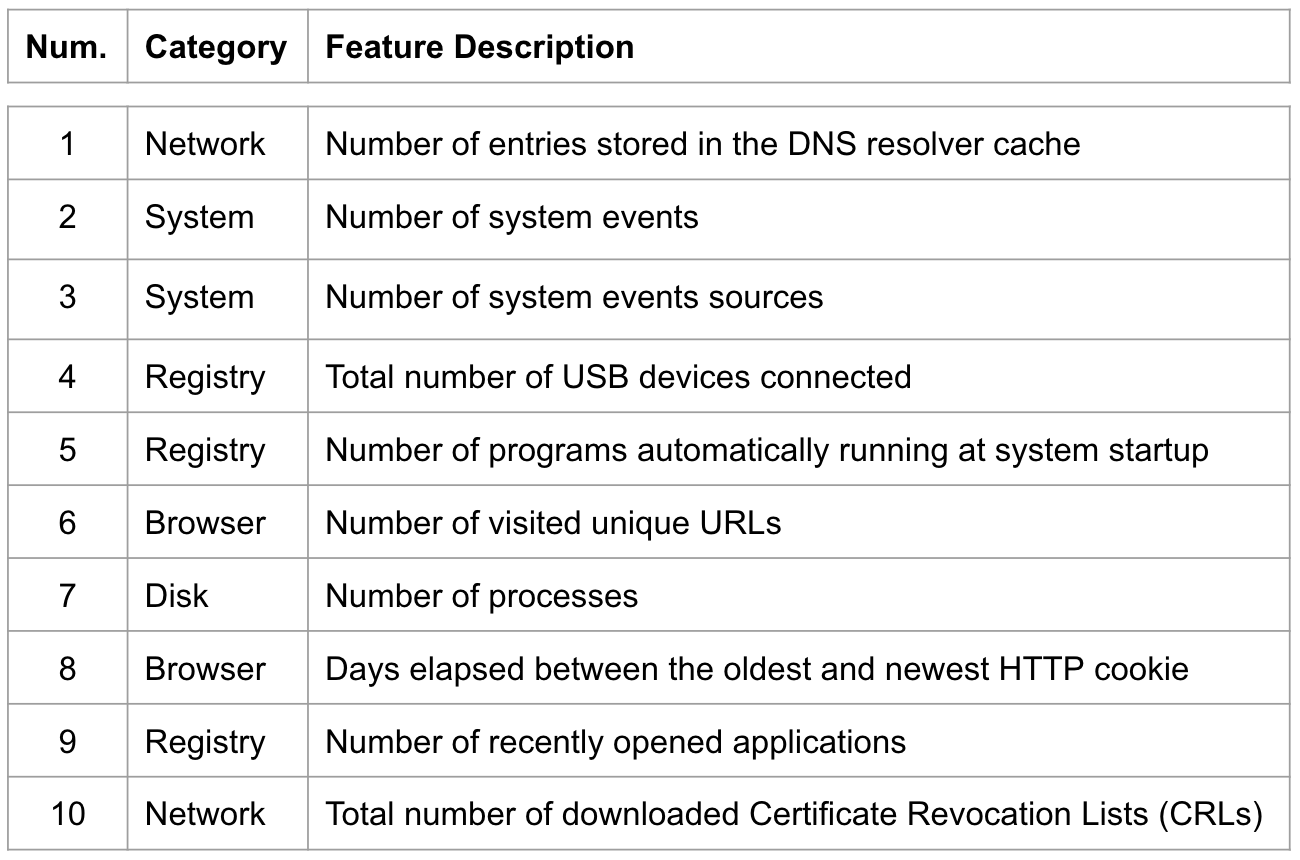
\includegraphics[scale=.5]{images/background5}
\caption{Prioritised list of features that evasive malware fingerprint to detect if running in analysis environments\cite{miramirkhani2017spotless}.}
\end{figure}
Evasive malware raise difficult challenges to malware analyst, slowing down the analysis process or even making it impossible. To ensure that this will not happen, the analyst must adopt suitable analysis strategies and employ tools tailored to help in neutralising evasive behaviours (see \autoref{sec:bluepill}).

\chapter{Employed Techniques}
\label{ch:chapter2}

\section{Information Flow}
\label{sec:informationflow}
How is it possible for an information system to prevent the leakage of sensitive data? This is the main problem that the field of security information flow tries to address. While there exist several solutions to limit the possibility of information disclosure (e.g., firewalls, access control) it is still difficult provide guarantees about the prevention of data propagation. In the world of cybersecurity, there exist a specific malware category namely, information-stealing malwares, which aims to collect sensitive information from the victim's computer for malicious purposes.\\

Information flow analysis is usually carried out through static analysis techniques which assess that the program does not leak any sensitive information\cite{smith2007principles}. Before starting the analysis, we need to define the \textit{information flow policy} as a triple $IFP = (O, SC, b, \leq)$ consisting of\cite{denning1977certification}:
\begin{itemize}
\item $O$ is a set containing program objects. Example of these objects can be anything involved into the program execution (e.g., program variables);
\item $SC$ is the set of \textit{security classes} or \textit{security levels};
\item $b$ is the \textit{binding} method responsible for assigning each object to the corresponding class. Usually, there exist two different methods for assigning an object into the appropriate class. The static binding expects the security level of a variable to be constant during the analysis while in dynamic binding, an object security class may change in accordance to the object content;
\item $\leq$ denotes the \textit{flow relation}. In particular, it specifies which are the legal flows between pair of classes. For example it is possible to write $L \leq H$, if and only if, information contained in class $L$ is allowed to flow into class $H$;
\end{itemize}
The pair $(SC, \leq)$ is said to be a \textit{lattice} of security classes, if all these three assumptions hold: $S$ contains a finite number of security classes, the flow relation is reflexive (i.e., $A \leq A$ is permitted) and the flow relation is transitive (i.e., if both $L \leq A$ and $A \leq H$ then it is legit to say that $L \leq H$). Moreover, it is possible to define the least upper bound $\top \in S \ s.t. \ A \leq \top, \ \forall A \in S$ and a greatest lower bound $\perp \in S \ s.t. \ \perp \leq A, \ \forall A \in S$. Usually, the least upper bound of a lattice is denoted by $H$ while the greatest lower bound is represented by $L$.\\
It is reasonable to think that any constant of a program, belongs to the least class $L$ indeed, constants do not refer to the sensitive content of any objects. On the other hand, if a constant is assigned to an object $a$ which is later transferred to object $b$ for which $a \nleq b$ then, \textit{only} in this moment, the flow of information must be prevented.\\

Information flows from object \textit{a} to object \textit{b}, denoted by $a \rightarrow b$, every time that information stored into \textit{a} is moved to \textit{b} or used for deriving information transferred to \textit{b}. A flow of information between two program objects can happen under different circumstances hence, it is possible to distinguish two types of flow:
\begin{itemize}
\item An \textit{explicit flow} of information $a \rightarrow b$ occurs when the value assigned to $b$ is the result of any set of operations applied on \textit{a}, independently of the value of \textit{a}. Examples of explicit flows are assignment operators, arithmetic operators, value-returning procedure calls.
\begin{lstlisting}[language=C++, caption=Example of explicit flow where the value of variable \texttt{b} is the result of an addition operation involving variable \texttt{a}.]
int explicit_function(int a){
	int b;
	/*The explicit flow of information happens here!*/
	b = a + 5;
	return b;
}
\end{lstlisting}
\item An \textit{implicit flow} $a \rightarrow b$ occurs when a set of operations creates a flow from some object \textit{c} to \textit{b} but the execution of the operations depends on the value of object \textit{a}.
\begin{lstlisting}[language=C++, caption=Example of implicit flow where the value assumed by variable \texttt{b} depends on the actual value of variable \texttt{a}.]
int implicit_function(int a){
	int c = func();
	int b;
	if (a == 0) {
		b = c;
	} else {
		b = c + 1;
	}
}
\end{lstlisting}
\end{itemize}
These are only the building blocks necessary to define information flow control in a system. Depending on why information flow security is enforced, the correspondent policy varies. Several solutions have been proposed to check information flow using \textit{type systems}, most of which to augment the security behind a programming language\cite{malecha2010more}. To carry out information flow security, any expression in a type system consists in a pair: a type (e.g., \texttt{int}) and a security label; then, based on this pair, the information flow policy can be either at compilation time, at runtime or even both\cite{sabelfeld2003language}.\\
The biggest drawback of typing systems is that they require to extend the underlying language thus, introducing changes in the syntax and semantic as well as a different compiler. Nonetheless, there exist other approaches and techniques, different from type systems, which allow to enforce information flow on a program.

\section{Taint Analysis}
\label{sec:taintanalysis}
We can imagine to put ourselves in the shoes of an hydrologist, who is in front of a river's source and would like to track the route taken by the river and find where it emerges. The problem that afflicts the hydrologist is that the river flows underground, with only its source visible from the surface. With a stroke of genius the hydrologist solved the issue by adapting the dye tracing method: he coloured the river's water with a dye, which acts as flow tracer once added to water. Therefore, to understand the exact point where the river emerges, he simply has to look for places where the coloured water resurfaces.\\

Similarly to the dye tracing method, \textit{taint analysis} is a technique to carry out information flow analysis. Instead of colouring river's water, we \textit{taint} the data of interest to understand the relationship between a program state and program location of interest\cite{Practicalbinaryanalysis}. Before proceeding in the description of the technique, we need to define what it means program state or location and also the way they can influence each other.\\

From an higher perspective, the main components of taint analysis are: 
\begin{itemize}
\item \textit{Taint sources}. They are the program or memory locations where identifying data of interest to be tracked. There is not any general rule to select sources rather, it is strictly bound to what we would like to achieve during the analysis. Indeed, depending on the chosen granularity, a taint source can be a system call or even a single instruction;
\item \textit{Taint sinks}. They are the program or memory locations which are checked to inspect if tagged data is present in the data flow. Just like taint sources, also taint sinks can vary depending on the case of interest and granularity. Typically, when tainted data reaches a sink during the analysis, an action is triggered which can be giving a warning, logging information about what happened or also prematurely terminating the analysis;
\item \textit{Taint propagation policies}\footnote{Without loss of generality, during the discussion the shorter term \textit{taint policies} will be used.}. They are responsible for propagating taint between a source and a destination\footnote{We would like to notice that a destination is not mandatorily a sink. Here a destination is intended to be any object influenced by tainted data.}. Among the three ingredients, a taint propagation policy is quite more complicated because it needs to account any relationship that might exist between input and output operands. For this reason, especially when talking about dynamic taint analysis (\autoref{sec:dta}) the implementation of taint propagation policies is left to a dedicated library.
\end{itemize}
Depending whether the analysis is performed statically or dynamically we have, respectively, static taint analysis or dynamic taint analysis.

\subsection{Static Taint Analysis}
As the name says, static taint analysis is performed statically, without executing the program. Since the benefit of statically analysing a program resides in a better code coverage, with static taint analysis is possible to identify program vulnerabilities or information flow leakage which may not come out during a normal execution. However, due to the lack of runtime information, this approach risks to be imprecise as it needs to approximate input and runtime objects\cite{arzt2014flowdroid}.

\subsubsection{Design Details}
Static taint analysis is a technique suitable for analysing both source codes and binary programs. Since the program is not executed, a Control Flow Graph (CFG) should be constructed for the application in question\cite{mumtaz2017critical}. A CFG of a program, is the graphical representation of the control flow of the application, showing how information propagates through the series of statements\cite{WhyProgr19:online}.

\begin{figure}[h!]
\centering
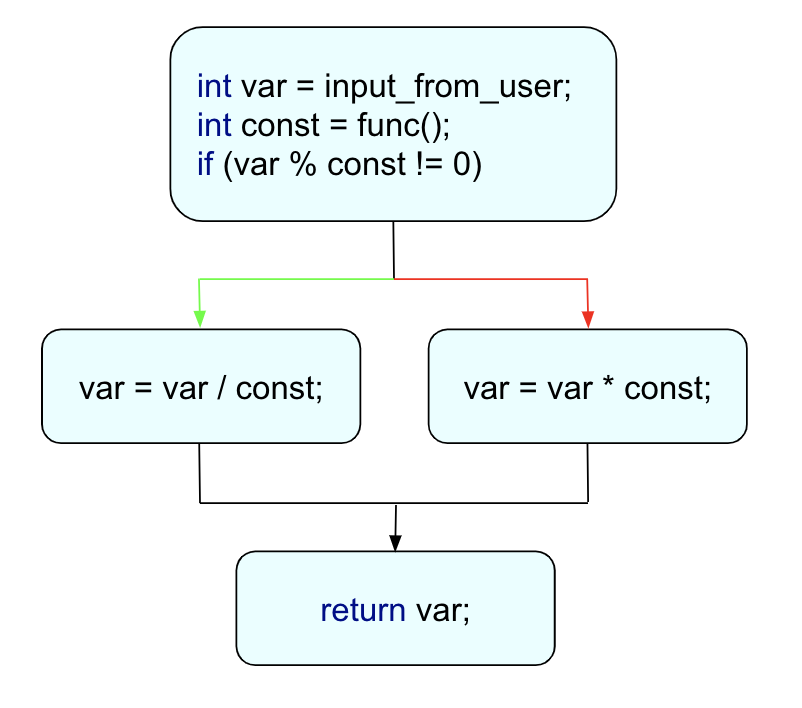
\includegraphics[scale=.5]{images/techn1}
\caption{Control flow graph of a simple \texttt{if-else} statement.}
\end{figure}

The taint propagation policy should handle all the possible statements:
\begin{itemize}
\item \textit{Write} statements can change the program state, such as assigning a new value to a variable $x \leftarrow const$ (where $const$ is a constant). Since on the right-hand side there is a constant, no taint policy would tag the left-hand side operand;
\item \textit{Control} statements (e.g.,\texttt{while}, \texttt{for}, \texttt{if}) affect the program counter and, consequently, the next statement executed. Usually, the program state does not include the program counter due to additional problems to be addressed (e.g., overtainting). However, in case it does include the program counter, the taint propagation policy must account cases when tainted data may change its value;
\item \textit{Read} statements are those which read the program state $x \leftarrow y$. In this situation, if the right-hand side operand is tainted then the left-hand side one will be tainted as well, otherwise it will not. When the left-hand side operand is assigned a value returned from a computation $x \leftarrow op(y, z)$ (e.g., arithmetic operation, function call) two strategies can be adopted: either tag $x$ as tainted or assign to $x$ the combination of $y$ and $z$ tags.
\end{itemize}
Usually, to keep track of every program variable, each one is represented as a tuple $(x, T)$ where: $x$ is the variable identifier and $T$ is the tag denoting if the variable is tainted or not. 

\subsection{Dynamic Taint Analysis}
\label{sec:dta}
Dynamic taint analysis (DTA) also known as data flow tracking (DFT), uses taint analysis technique while the program is executing. Even though this means having smaller code coverage, at the same time it allows a more precise analysis. Indeed, we now have access to all runtime information like the value of memory addresses as well as memory content.

\subsubsection{Design Details}
The first aspect to be discussed is the \textit{taint granularity} which identifies the tag data unit. Defining the granularity to be as small as single bits, enables us to be more accurate and to perform a very fine-grained data flow tracking. For example, let's consider the propagation of taint through a bitwise operation where just one of the two operands is tainted.

\begin{figure}[h!]
\centering
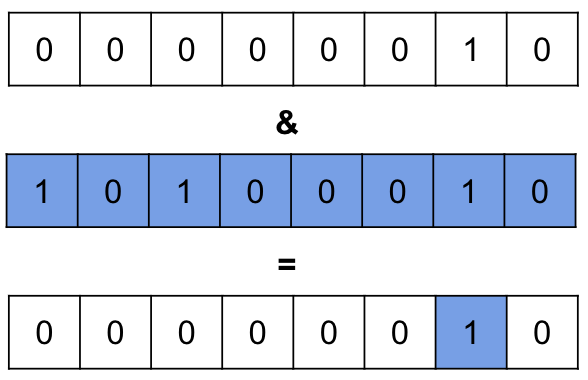
\includegraphics[scale=.5]{images/techn2}
\caption{Bitwise AND operation between two bytes. Each box is the memory cell where the bit is stored: white cells indicate that the bit is untainted while those azure are tainted. In this case, the propagation is performed with bit-granularity.}
\end{figure}

Being a bitwise operation, the only bit set to $1$ in the result will be the second from the right. Moreover, given that the system works with bit-level granularity, even if the first operand is completely tainted, only the second bit of the output will be tainted. Vice versa, using a larger granularity, brings the data flow tracking system to be less accurate and thus, more error-prone.

\begin{figure}[h!]
\centering
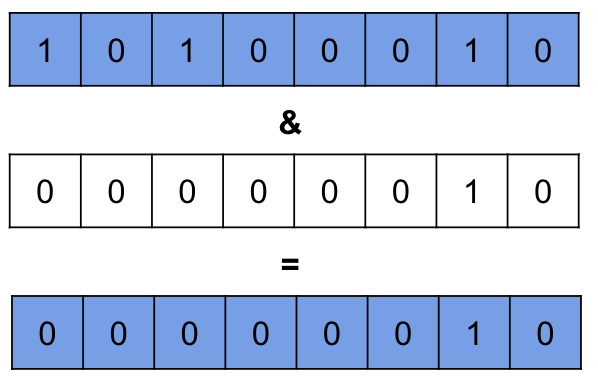
\includegraphics[scale=.5]{images/techn3}
\caption{Bitwise AND operation between two bytes, one of which is tainted. Here, the system adopts byte-granularity propagation.}
\end{figure}
\newpage
The difference that stands out is that, even if the two input operands are exactly the same, in the latter case the entire output byte ends up being coloured. Working at byte-level granularity, the system is not able to taint just a single bit but it will taint at least, one byte.\\
Even if a byte-level DTA system is less accurate than one adopting bit-level granularity, in practice it is the most adopted. The reason is the complexity which would be required to track taint propagation for a single bit, leading to unacceptable performance.\\

Another aspect which needs to be addressed when developing a DFT system, is related to the concept of \textit{taint colour}. A DFT system usually supports two operating ways:
\begin{itemize}
\item Using a binary tag as taint colour. Any system which uses a binary value to taint an object, is only capable to identify the program state as tainted or not, without giving any other meaningful information about the source of taint; 
\item Adopting set of taint colours. Using more than a simple binary value to taint an object, allows the system to provide further insights about the correspondent source. Indeed, if the two input bytes in the figures above were both tainted with different colours, then the output byte would have been coloured with a combination of the two input taints.
\end{itemize}

\begin{figure}[h!]
\centering
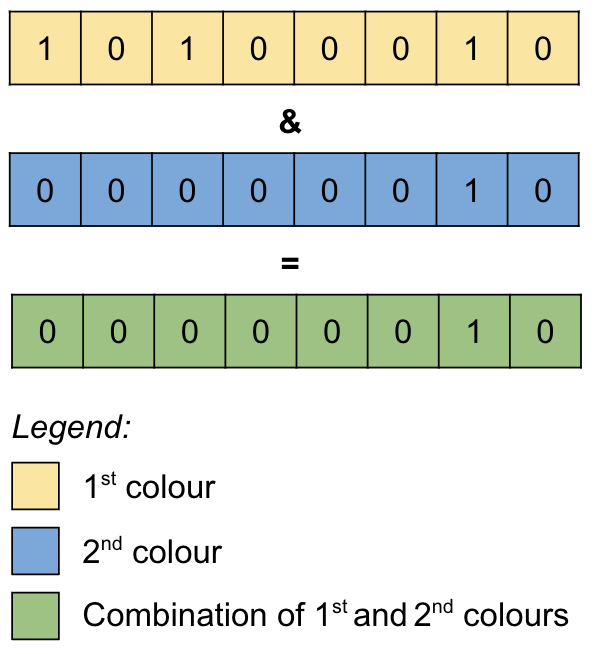
\includegraphics[scale=.5]{images/techn4}
\caption{Bitwise AND operation between two bytes, both of which are tainted with different colours. Here, the system adopts byte-granularity propagation and supports the combination of different taints.}
\end{figure}

\newpage
However, not all that glitters is gold because a system supporting multiple taint colours with the possibility of combining them, is more complicated than a system of the first type. Indeed, assuming to work with a DTA system adopting byte-level granularity:
\begin{itemize}
\item In case of a single taint colour, the system would need to store just a single bit for each byte of memory. Therefore, this bit will be $1$ if the correspondent memory byte is tainted otherwise it is $0$;
\item On the contrary, if the system allows to combine tags supporting a set of different taint colours, it needs to store and manage more information for each memory byte.
\end{itemize}
As already mentioned in \autoref{sec:taintanalysis}, the taint policy is a central building block in the design of any taint analysis system. In particular, it describes how the taint is propagated for all possible types of operations. Nonetheless, a system supporting different taint tags, must also design a policy for merging colours when multiple taints flow in a single memory location\footnote{Here the term memory location is generic and depends on the granularity level of the system.}.

\begin{figure}[h!]
\centering
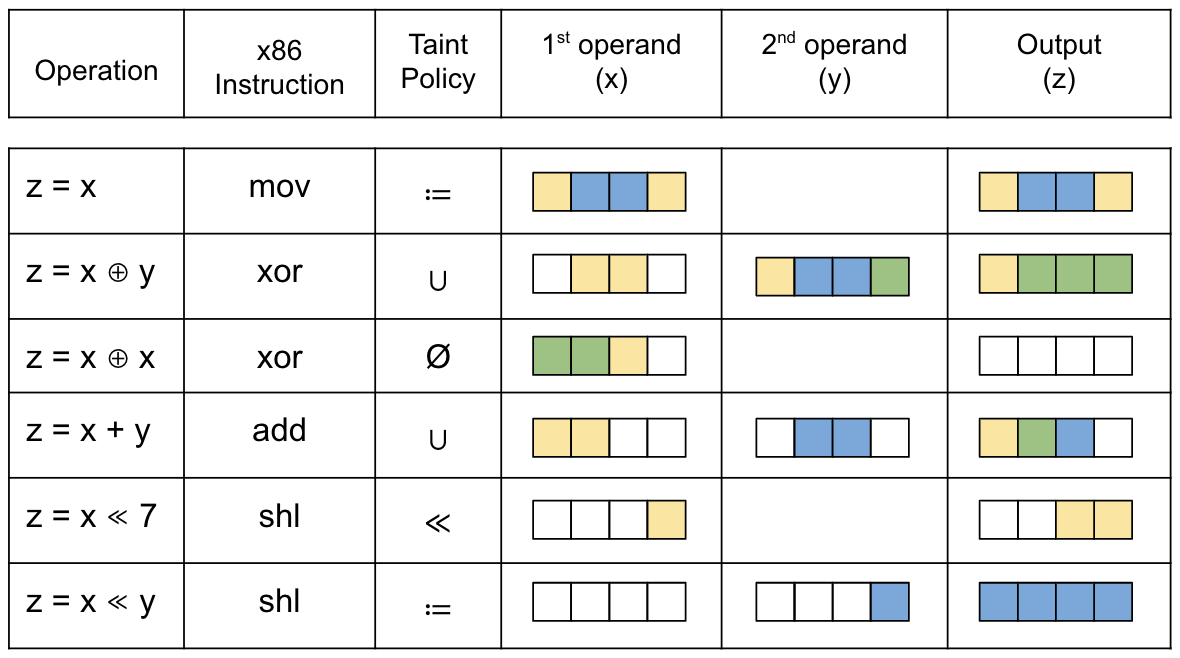
\includegraphics[scale=.6]{images/techn5}
\caption{Example of possible taint propagation policies employed in a byte-granularity DTA system.}
\label{fig:techn5}
\end{figure}

For assignment operations, the taint policy is immediate: if the right-hand side operand is tainted, propagate its colour to the left-hand side, otherwise do nothing.\\
While it is easier to identify cases when a variable changes its state from untainted to tainted, it is not immediate to think of situations in which an object should change its state from tainted to untainted. When designing the taint policy, the third operation in Figure \autoref{fig:techn5} needs more attention. Despite the second case where input operands are different, here the \texttt{xor} is carried out using the same object for both input arguments. It is well-known that the output of such operation is $0$ but it not as clear which policy should be adopted. Usually, since the content is zeroed, the same happens to the respective tag.\\

As the name says, a DFT system is designed to track the data flow during program execution. However, we have already seen in \autoref{sec:informationflow} that information can also flow implicitly. The condition according to which the data flow becomes influenced by an implicit flow, is when a dependency is set between tainted data and the condition of a control statement.

\begin{lstlisting} [language={C++}, label={lst:implictflow1}, caption={Function where tainted data can cause implicit flow.}]
/*
* Example 1: simple case of implicit flow caused by the involvement
* of the tainted variable seed in the condition of the if statement.
*/
int example_1(int seed) {
	int res;
	if (seed % 2) {
		res = 0;
	} else {
		res = 1;
	}
	return res;
}
\end{lstlisting}
\begin{lstlisting} [language={C++}, label={lst:implictflow2}, caption={Function where tainted data can cause implicit flow. However, compared to the first example, here the complexity level is higher.}]
/*
* Example 2: more complex case of implicit flow where the the tainted
* variable seed is involved in nested control flow statements.
*/
int example_2(int seed) {
	int res[10];
	for (int idx = 0; idx < seed || idx < 10; idx++) {
		if (idx == seed/2) {
			res[idx] = func_1();
		} else if (idx == seed-1) {
			res[idx] = func_2();
		} else {
			res[idx] = 0;
		}	
	}
}
\end{lstlisting}

Looking at the first example in \ref{lst:implictflow1}, if the variable which appears in the \texttt{if} condition is tainted, then we could also be interested in tainting the value of \texttt{res}. Although it may seem simple, only one variable within the body of a control flow statement is rare. Indeed, more often, within the body there can be several memory objects or even nested control flow statements (see example in \ref{lst:implictflow2}).\\
Different research works\cite{graa2012detecting}\cite{clause2007dytan}\cite{chen2011dynamic} tried to address the problem of control flow dependencies while performing dynamic taint analysis. The main ones and those that reached the greater success, use a combination of static and dynamic analysis:
\begin{itemize}
\item A first phase of static analysis is needed to identify program locations in which a possible tainted object could influence the decision in a control statement. Usually, this is accomplished by resorting to an analysis of the CFG of the program or through additional data structures like the post-dominator tree to enhance the precision;
\item The second step consists in applying data flow tracking and accommodate control flow dependencies using observations from the previous phase. The most commonly adopted policy, consists in colouring all the memory regions involved within the body of the branch.
\end{itemize}
Whether it is meaningful to track the control flow or not, depends on the application domain. Furthermore, it is known that a DTA system enabled to manage implicit flows produces a greater number of false positives than a similar system that only tracks data flows.\\

Commonly, a DTA system, raises too many false positives when values end up tainted even though they should not. This causes the system to trigger an alert when, in practise, it is not necessary. In the field of dynamic taint analysis, this problem is known under the name of \textit{overtainting} and the main cause comes from implicit flows. This is the reason why only few systems focus on implicit flow tracking.\\
Conversely, a DTA system which does not taint a value when, in practice it should do, suffers from \textit{undertainting}. Consequences of undertainting are the possibility for a value, to pass unnoticed even if it is influenced by a tainted object. The main causes are:
\begin{itemize}
\item The taint policy does not take into account specific corner cases. For example, when adding two (tainted) bytes it may happen to have an overflow bit in the second least significant output byte. To patch this corner case, the policy should explicitly look for overflow bits and color them appropriately. Although the accuracy of a DTA system would increase, many of them do not handle these special cases for a faster taint propagation;
\item While control flow tracking is known to cause overtainting, at the same time only performing data flow tracking entails to undertainting issues.
\end{itemize}
Virtually any system, each one with a different degree, suffers from both undertainting and overtainting. In fact, avoiding these problems while maintaining good performance is practically impossible.
\newpage
\section{Code Instrumentation}
In software engineering, the most adopted technique for analysing software is through debugging. This is usually done by a software engineer during the development to identify where the program fails in order to fix that failure. In a situation like that, the debugging session can be enhanced by the availability of source code which is by no means obvious.\\
In this context, the task of a malware analyst is similar to the one of a software engineer even though it is more tedious. Indeed, it is already difficult to recover the binary related to a malware, let alone the source code. Besides, a malware analyst has to deal with software which is often able to detect when it is being analysed (e.g., evasive malware in \autoref{subsec:evasivemalware}) hindering his job. Therefore, it is of primary importance for the analyst to have adequate tools through which monitoring the malware behaviour as well as extracting useful information.\\ 

\textit{Code instrumentation} is a technique which allows to insert additional code fragments into a program with the objective of monitoring or modifying its behaviour. The code inserted through this technique is called instrumentation code while the point where it is added takes the name of instrumentation point.\\
In source code, the instrumentatio fragment is injected right before the program is compiled\cite{geimer2009generic}. Thanks to the availability of source code, the instrumentation process can place additional code not only at the level of functions but also at loop level or even at each statement. While instrumenting source code can be useful especially for testing and debugging purposes, it is impossible to have the source code of malicious software at hand. Thankfully, there exist tools which allow to carry out instrumentation on binary executables and depending on whether the instrumentation process is static or dynamic, we can distinguish between:
\begin{itemize}
\item \textit{Static binary instrumentation (SBI)} also known as \textit{binary rewriting}, carries our the instrumentation process by rewriting the input binary. Compared to other instrumentation approaches, it covers only the input binary file but at the same time, it has better performances\cite{ermakov2017static};
\item \textit{Dynamic binary instrumentation (DBI)} allows to instrument the program while it executes, modifying the binary on the fly. While in the static instrumentation it is possible to rewrite the file only once and run it multiple times, the dynamic approach needs to parse and modify the program at each execution, leading to an higher overhead.
\end{itemize}

\begin{figure}[h!]
\centering
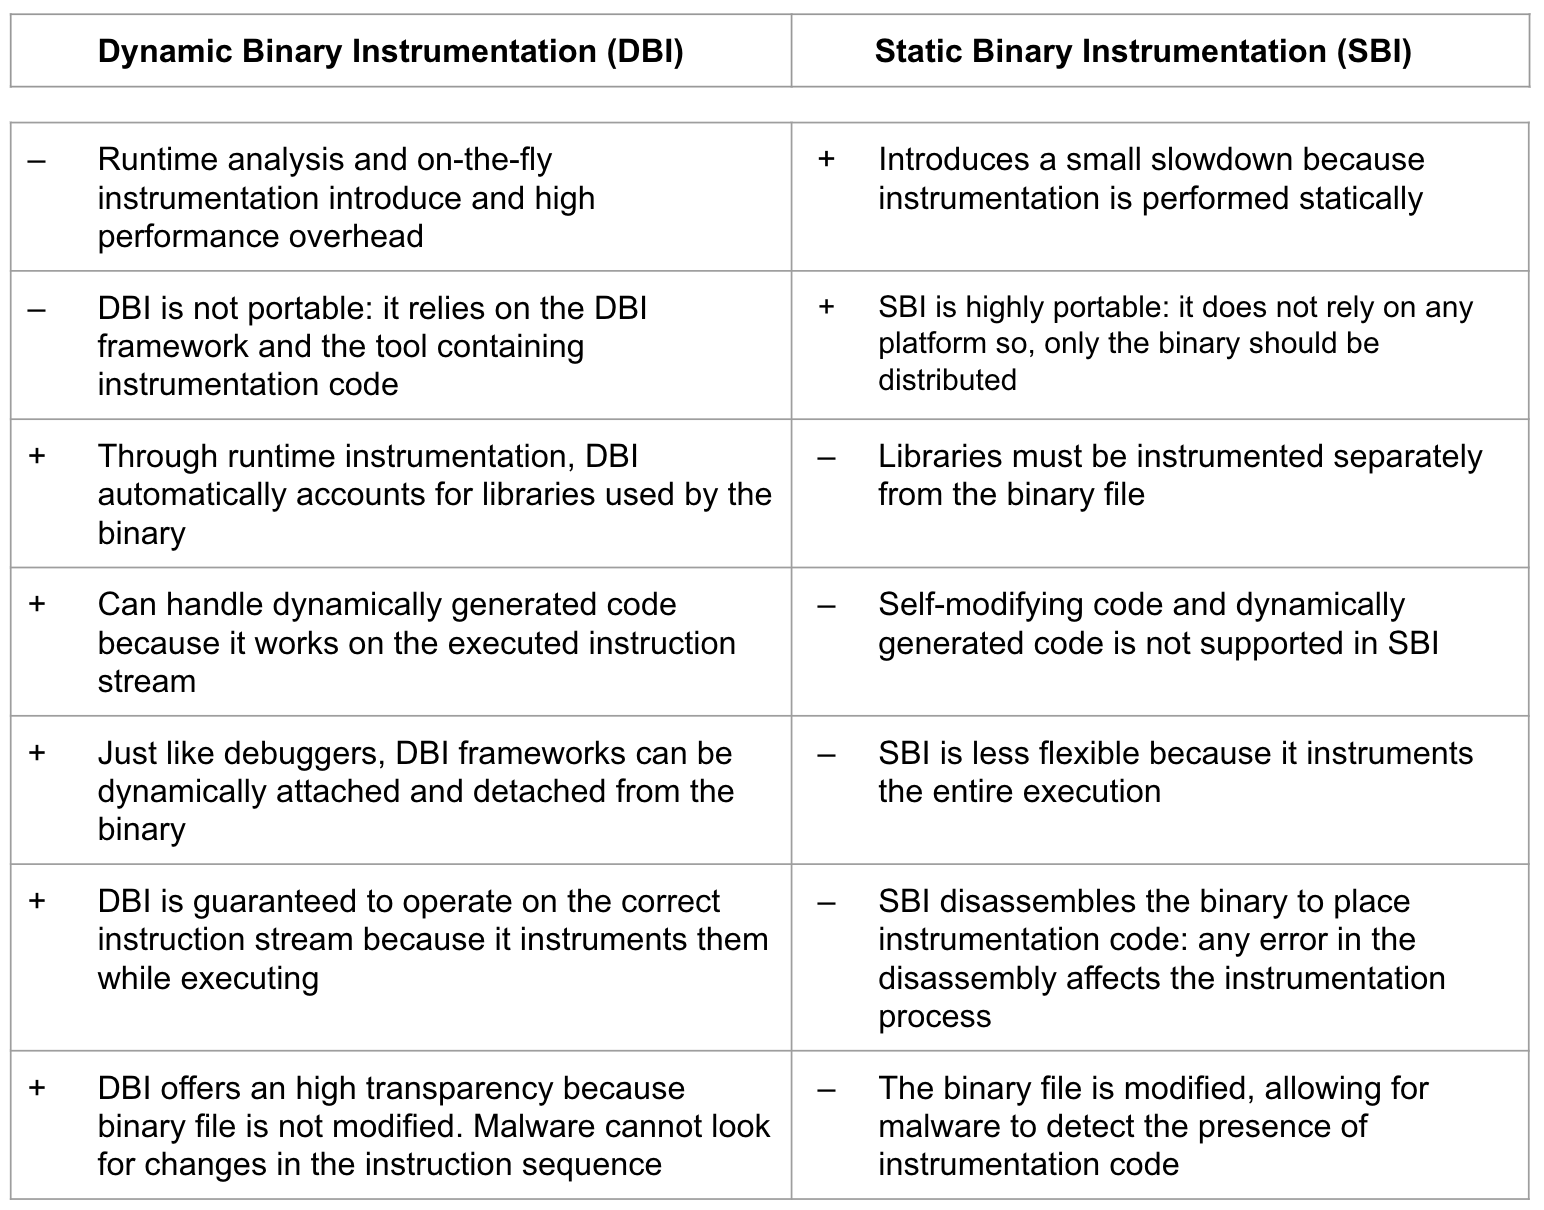
\includegraphics[scale=.5]{images/techn6}
\caption{Table showing advantages (+) and disadvantages (-) of Static and Dynamic Binary Instrumentation techniques.}
\end{figure}
\newpage
\subsection{Dynamic Binary Instrumentation (DBI)}
\label{subsec:dbi}
Rather than static binary instrumentation which requires to disassemble and rewrite the binary, DBI frameworks parse the instruction stream as the binary executes. This is a convenient feature for users who do need to recompile the program for each different execution\cite{nethercote2007valgrind}. DBI techniques allow to monitor or even alter the execution of software through the insertion of probes or user-defined routines, directly into the running executable\cite{d2019sok}. Moreover, the whole procedure does not require either accessing the source code or changing the binary executable at runtime.\\
A DBI framework is the application executing binary programs under virtualised environment giving, at the same time, introspection capabilities in a programmatic manner. The DBI system offers a set of APIs through which it is possible to develop DBI tools that is, user-defined programs specifying:
\begin{itemize}
\item The instrumentation code, which includes code fragments in charge of identifying the right instrumentation points where to insert probes or user-defined routines;
\item User-supplied code. This is usually in form of routines which define the monitoring logic or that alter the program execution.
\end{itemize}
Being provided in a programmatic way, before actually starting to analyse the binary, instrumentation and user-supplied code need to be plugged-in the DBI system. Thus, the initialization step (i.e., through the framework initialization function) is required by the framework for understanding what (i.e., instrumentation code) should be instrumented and how (i.e., analysis code). Even though the architecture of a DBI framework is highly complex and optimized, its high level approach consists of four steps: 
\begin{enumerate*}[label=\roman*),itemjoin={,\quad}]
\item fetch code from the binary
\item instrument these code blocks
\item compile them
\item finally execute.
\end{enumerate*}
Each time a new code block\footnote{Here the concept of code block is generic and is independent from the granularity at which DBI systems work.} is available, the DBI system fetches it from the process and instruments the block following the directives given at initialization phase. Before actually executing it, the code must be compiled according to the underlying ISA\footnote{ISA stands for Instruction Set Architecture (e.g., x$86$).}. The compilation process is held using JIT\footnote{Although the compilation process is performed before execution, just-in-time (JIT) compilation involves compiling code on-the-fly while the program is running. It is the most adopted way through which DBI frameworks handle dynamic compilation.} compilers that optimize the instrumented code (i.e., original code plus instrumented code) storing it in the code cache. The purpose of a \textit{code cache} in a DBI framework is twofold:
\begin{itemize}
\item The first objective is to run code. Whenever new code is fetched, instrumented and then compiled, it is inserted into the code cache ready to be executed. Thus, the system runs instrumented code from the code cache;
\item The second goal is that of any other cache namely, to speed up execution. Before fetching a new code block from the process, if that block was previously instrumented, then it is already cached and ready to be executed. This is only one of the optimizations which DBI frameworks adopt to reduce the performance overhead.
\end{itemize}
The JIT compiler also modifies control flow statements to give the control back to the DBI system avoiding to continue the execution of not instrumented code. The alternative to JIT-based dynamic instrumentation is the probe-based approach: program instructions are dynamically substituted with trampoline code that jumps to instrumented instructions\cite{buck2000api}.\\
The most common JIT-based DBI frameworks are: Valgrind\cite{nethercote2007valgrind}, DynamoRIO\cite{bruening2012transparent} and Intel Pin\cite{luk2005pin}. While all of them share the same high-level approach described above, each one may adopt different implementation strategies.

\subsection{Intel Pin}
Intel Pin is a dynamic binary instrumentation tool available on all the major operating systems and supporting executables compliant to the IA-32 and IA-64 architectures. The goal of Pin is to provide an instrumentation framework through which developing a wide range of program analysis tools. The distinctive features of this framework are the following:
\begin{itemize}
\item \textit{Portability}. Pin APIs allow to access fine-grained information about the underlying architecture, abstracting away any low-level implementation detail;
\item \textit{Efficiency}. The framework implements several optimizations which set Pin apart from its competitors;
\item \textit{Ease-of-use}. It automatically performs tasks like instruction inlining without requiring external actions (i.e., manual intervention from users);
\item \textit{Transparency}. When running under Pin, the instrumented application has the same view on instructions, registers and memory as it would not be executed under Pin;
\item \textit{Robustness}. Given the delayed code analysis, Pin can monitor several behaviours (e.g., dynamically generated code) which SBI alone cannot do (e.g., indirect branches).
\end{itemize}
A DBI tool developed through Pin is called \textit{pintool}. According to its software architecture, when an instrumented application is running, there are actually three involved programs: the application, the pintool and Pin. Even though they have the same view on address space, no library is shared.

\begin{figure}[h!]
\centering
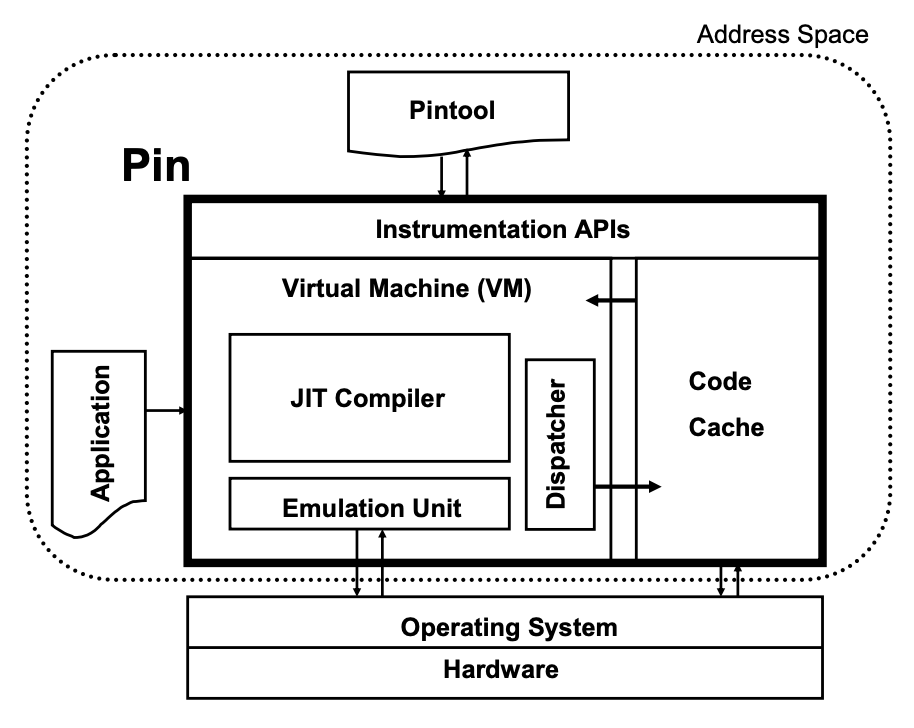
\includegraphics[scale=.7]{images/techn7}
\caption{Software architecture of Pin DBI framework.}
\source{"Pin: Building Customized Program Analysis Tools with Dynamic Instrumentation."}
\end{figure}
\newpage

The process of instrumenting an application consists of the following steps:
\begin{enumerate}
\item The injector module is responsible of loading Pin into the address space of the target application;
\item Pin accomplishes the initialization phase (\texttt{PIN\_Init()}) and loads the pintool;
\item The pintool initialises itself and request to Pin to load the target application (\texttt{PIN\_StartProgram()}).
\end{enumerate}
Pin defines \textit{analysis routines} as the user-supplied procedures injected through \textit{instrumentation routines} which, in turn, determine where analysis code should be inserted. Analysis code can vary from simple monitoring procedures to altering program state by changing register and memory content or overwriting process memory.\\
Pin uses a JIT compiler to do on-the-fly instrumentation exactly as described in \autoref{subsec:dbi}. Even though Pin fetches and compiles code at trace (e.g., set if instructions starting at a branch target and ending with unconditional jumps) granularity, the framework allows to analyse also procedures (e.g., function or system call), images (e.g., dynamic link library) and of course, instructions. When a trace exits, the virtual machine is in charge of resolving the target address, generating a new trace if not already available and resume execution at that trace.\\
Adopting probe-based dynamic instrumentation would go against Pin design choices. The probe-based approach is not transparent because program instructions are overwritten in memory, it is not robust for architectures where instruction sizes vary because it is not feasible to use trampolines larger than original instructions and lastly ,it is not efficient due to different levels of branches to implement trampoline code. Instead, through the JIT compiler, Pin adopts several optimizations to boost the performances of the tool, some of which are as follows:
\begin{itemize}
\item Linking the exit of a trace to the beginning of the next one. Trace linking is an optimization allowing to bypass the overhead introduced by the VM when a trace is already available. For direct control flow changes, Pin patches the target address to jump directly to the trace while, for indirect control transfers the idea is to keep a set of possible target addresses. Specifically, Pin adopts function cloning to handle \texttt{ret} instructions and target chaining for the remaining indirect control flow statements;
\item Allocating registers rather than obtaining extra ones. Often during JIT compilation, it happens to use CPU registers. However, when performing instrumentation, the JIT compiler must not overwrite registers currently used by the application. To solve this problem, Pin adopts an efficient linear scan algorithm to perform register allocation\cite{poletto1999linear} for both the application and the pintool. Even though allocating register is necessary, spilling them too often is inefficient. To reduce register spilling, Pin adopts several strategies like the analysis of register liveness information between the exit point and the beginning of traces;
\item Analysis code optimization. Usually, before actually execution analysis code, the JIT compiler invokes a bridge procedure which stores caller-saved registers and transfers execution to the analysis routine. Despite this is the standard procedure, some analysis routine can be optimized further. This is the case of analysis procedures performing simple task that pin inlines avoiding the overhead introduced by the bridge stub.
\end{itemize}
Although dynamic binary instrumentation is used in several software engineering domains including binary optimisation and program analysis, it is also employed in wide range of security fields. Specifically, some of the most relevant domains include reverse engineering (e.g., code de-obfuscation), vulnerability discovery (e.g., memory overflow), malware analysis (e.g., malware detection) or also information flow security (e.g., symbolic execution and taint analysis frameworks).

\section{Blue Pill}
\label{sec:bluepill}
In \autoref{subsec:analysisenvironment} we already presented the necessity for a safe environment where analysing malicious software. The ability to isolate malicious actions is of course, a crucial feature which should characterise any analysis environment even though, it is not enough. Along with several other programs, the analysis system represents the tool which allows the analyst to go through malware dissection thus, it must be effective in doing so.\\
Given the number of malware categories in the wild, flexible and transparent analysis systems are preferred because easily adaptable. The ability of security professionals in developing techniques to dissect and profile the malware behaviour, meets the cunning of malware writers who continually develop new anti-analysis hacks against malware dissection (see \autoref{subsec:evasivemalware}). Often before harming the victim, malicious samples seek the presence of any analysis system (e.g., virtual machines, debuggers) and, if so, they either act as benign or even try to bypass it. Supporting the analyst against evasive malware behaviour, providing at the same time fine-grained control during its dissection, would make the whole analysis process less time-consuming.

\subsection{Approach}
Despite automatic systems provide helpful indicators, a significant chunk of work is carried out by analysts who come-up with more in-depth information about those findings. In this context, \textit{BluePill}\cite{bho} is a dynamic analysis system designed to fulfil transparency requirements meanwhile offering fine-grained capabilities needed for dissection. The features that distinguish BluePill from its competitors are:
\begin{itemize}
\item Robustness against anti-analysis (adversarial) techniques and stealthiness when altering data or instructions during execution;
\item Precise control capabilities over malware execution;
\item Extensibility to include new countermeasures to neutralise anti-analysis behaviours (e.g., found during dissection).
\end{itemize}
\newpage
BluePill is capable of deceiving the malware to have infected the victim through the following schema:
\begin{enumerate}
\item It observes all kind of operations (e.g., fingerprinting) which may trigger anti-analysis techniques;
\item It tests if the outcome of these environmental checks are not compliant with the analyst choice;
\item It replaces results that differ from expectations, crafting the actual value seen by the malware.  
\end{enumerate}
This paradigm is as simple as effective in managing all categories of environmental operations. Indeed, it supports both environmental checks which are independent from the outcome of previous operations (i.e., stateless) as well as those which depend on previous observations (i.e., stateful).

\subsection{Architecture}
BluePill is designed on top of a DBI framework strengthening its robustness, stealthiness, extensibility and precision. The current implementation of BluePill supports both IA-32 and IA-64 Windows executables using Intel Pin as dynamic binary instrumentation system. Even though it is actually implemented on Pin, there is not any particular operation tied to it, making BluePill portable to different DBI systems. Moreover, BluePill architecture is composed of different layers which, on top, share the observe-check-replace layer.

\begin{figure}[h!]
\centering
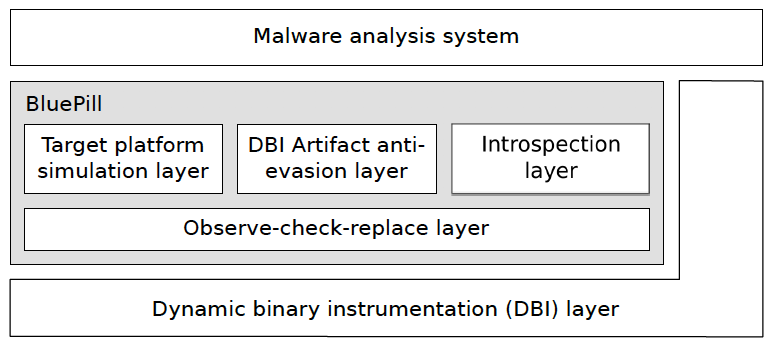
\includegraphics[scale=.6]{images/techn8}
\caption{Bird's eye view of BluePill architecture.}
\source{"On the Dissection of Evasive Malware."}
\end{figure}

\subsubsection{Target Platform Simulation Layer}
\label{subsec:targetplatformsimulation}
The \textit{target platform simulation layer} is responsible for hiding artifacts through which any malicious software can detect the analysis environment. Specifically, it alters the distinctive features of a virtual machine like VirtualBox mounting a Windows image rather than any other VM or hypervisor. The artifacts on which the layer focuses on, are both related to environment fingerprinting and specific to sample execution.\\
Environmental artifacts altered by the system are:
\begin{itemize}
\item Instructions whose behaviour depend on whether they are virtualised or not (e.g., \texttt{sidt} on VMware). Even some data structures may have different content whether they are virtualised or in a native system;
\item Hardware characteristics which make virtualised systems recognisable from native ones. This list includes CPU model, number of adapters, MAC address family, among others;
\item Divergences in Windows images. Specifically, when a Windows image is installed into a VM or hypervisor, the latter includes distinctive artifacts like registry entries, files and processes;
\item User fingerprint. By looking at artifacts like browser history and recently opened file, malware can estimate the "level of use" of an OS. Through this estimation, a sample may understand whether the underlying OS is installed in a virtualised environment or not;
\item Presence of specific applications. The most common evasive behaviour adopted by a malware is checking whether in the target system, there are installed specific analysis tools (e.g., debuggers, anti-viruses).
\end{itemize} 
A different category of artifacts are those which should be altered only during the execution:
\begin{itemize}
\item Library calls or system calls which access specific registry keys, files or drivers;
\item Instructions like \texttt{cpuid} and \texttt{rdtsc} can reveal hardware characteristics as well as the elapsed time;
\item Process-specific data structures like the Process Entry Block (PEB) let a sample understand if it is being debugged;
\item Output of queries to the Windows Management Instrumentation (WMI).
\end{itemize}
Windows, as any other operating system, exposes different functionalities to implement timers or to retrieve time information (e.g., current time). As already discussed in \autoref{subsec:evasivemalware} there exist several time-related tricks through which malware author can discover virtualised environments. A sample can go beyond just performing multiple sleep calls, monitoring the elapsed time between each of them to detect possible fast forward mitigations. Therefore, patching individually each call could expose inconsistent information because different time sources would not be synced.\\
BluePill counters time-related tricks proceeding in two steps. At first, when any time-stalling call is invoked, the requested amount of time is accumulated while the execution is delayed only for few milliseconds. Later, when the timer expires or the sample checks for the elapsed time, the accumulator is used to fake the results. In addition to countering time-stalling techniques, this scheme allows to hide the overhead introduced both by dynamic binary instrumentation and by the analysis carried out on top of BluePill.

\subsubsection{Introspection Layer}
The \textit{introspection layer} uses PinADX\cite{lueck2012pinadx} for exposing to debuggers a view of the program as if DBI related arifact (e.g., JIT compilation) were not present. This scheme allows to hide breakpoints during the execution, thus preventing evasion techniques based on software breakpoints or divergences in instruction sequences.\\
BluePill introduces also a new method which allows to apply code patches during debugging. Specifically, it allows the analyst to change arbitrary length code while debugging a sample. This is possible by JIT-recompiling the involved instructions and introducing trampolines which the program cannot detect since the DBI scheme points them to the original addresses (i.e., not jitted addresses). In the end, this mechanism allows to alter instruction of a malicious sample, while being stealthy against anti-tampering and anti-checksumming techniques.

\subsubsection{DBI Artifacts Anti-Evasion Layer}
The \textit{DBI artifacts anti-evasion layer} is in charge of hiding artifacts which may expose the presence of an underlying DBI system. Indeed, a painstaking malware author can detect its presence through several techniques like checking for runtime overhead, leaking the instruction pointer or also verifying the consistency of memory permissions. BluePill provides countermeasures for all these attacks including detections based both on time and on debugging artifacts.\\
The fast forwarding mechanism discussed in \autoref{subsec:targetplatformsimulation}, is already an effective countermeasure against anti-DBI techniques that check for runtime overhead.\\
The introspection layer already prevents anti-tampering techniques but a malware can still look for debugging artifacts. To accommodate these situations, if an exception is caught, BluePill allows passing the exception to the sample. This can happen, for example, when the analyst temporarily detaches the debugger and waits for it to reattach before resuming the execution in the malware handler. Moreover, to hide completely the presence of a debugger, BluePill also changes the \texttt{BeingDebugged} byte into the PEB.\\

Blue Pill framework already comes with the support to dynamic taint analysis. Since Blue Pill is a Pintool, the best choice would be implementing the DFT system using APIs offered by Intel PIN.

\section{libdft}
Dynamic taint analysis refers to the technique that consists in tagging and tracking data of interest as they propagate during program execution. At this point, it is necessary to introduce a framework or library that implements the logic behind dynamic flow tracking.\\
libdft\cite{kemerlis2012libdft} is a dynamic data flow tracking library implemented on top of Pin DBI framework. The main characteristic that distinguishes this library from similar works in this field\cite{bosman2011minemu}\cite{qin2006lift}, is the high customization and ease with which it can be modified. Indeed, thanks to the large set of APIs exported by the library, it is possible to implement a DFT tool in a simple and effective manner.

\subsection{Design Choices}
We already discussed the functionalities offered by a dynamic binary instrumentation framework, especially Intel Pin. Given the granularity at which the DBI framework allows to insert analysis code, a tool enabled with libdft, can use three kind of data source or data sink: function calls, system calls and process instructions. After deciding what should be a source and sink, the user can place callbacks routines to inspect the data flow as well as tag or untag data.

\begin{figure}[h!]
\centering
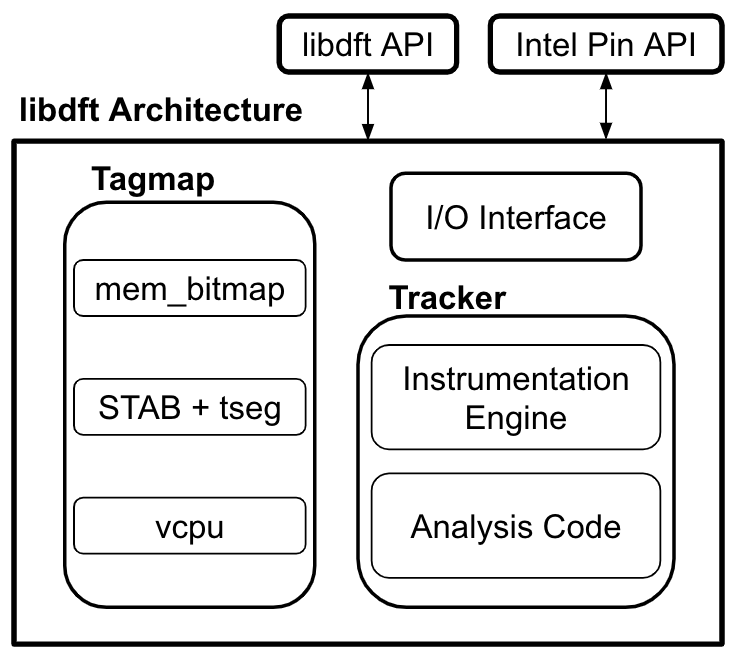
\includegraphics[scale=.6]{images/techn9}
\caption{Bird's eye view of libdft architecture.}
\end{figure}

To taint data, libdft maintains a process-wide data structure (\autoref{subsubsec:memorymap}) storing tags for each program memory location. The two design choices which allow to determine the format of a tag are the following:
\begin{itemize}
\item The granularity adopted for performing tagging operations, that is, the tag granularity. libdft works at byte-level, which offers the best trade-off between fine-grained tracking and performance;
\item The size used to store a tag, namely, the tag size. The larger the size of a tag, the higher the number of tags which allow to uniquely identify different kind of data. Nonetheless, the larger the size of a tag, the higher memory storage is required for each byte. libdft offers two tag sizes: a bit tag, which allows mark a byte either tainted or not and a byte tag, for attaching $8$ distinct colours to each byte.
\end{itemize}
After defining the format of the tag, a propagation policy is required to correctly drive the tag through program locations. The way libdft propagates each tag, is by inspecting every instruction which leads to a possible data dependency among its operands (\autoref{subsubsec:taintpropagationlogic}). Then, based on the dependency originated by the instruction, a suitable analysis function is injected to perform the tag propagation logic.

\subsection{Implementation Details}
The core data structure that holds every tagged byte and around which the data flow tracking logic works, is called \textit{tagmap}. Internally, the tagmap is divide into two smaller memory maps: one keeps tags for each memory byte allocated by the program while the second map is used to store tags for CPU registers.

\subsubsection{Memory Map}
\label{subsubsec:memorymap}
Depending whether bit-size or byte-size tags are used, libdft allocates a different kind of data structure.
\begin{itemize}
\item When byte-size tags are used, they are stored in a dynamically allocated segment called \texttt{tseg}\footnote{\texttt{tseg} stands for \textit{tagmap segment}. The two terms will be interchangeably used during the discussion.}. Each time the program allocates memory or requests a memory mapping, libdft intercepts the call and allocates an equally sized \texttt{tseg}.\\
When using tags of this size, the shadow memory needed by libdft has the same size of the memory allocated by the program. The virtual address space which the OS usually reserves to processes is $3$GB\footnote{This number refers to $32$-bits versions of Windows OS\cite{VirtualA15:online}.} thus, it would be practically impossible (and physically impossible for $32$-bits OS which can have only $4$GB addressable memory) to allocate a-priori the same amount of shadow memory. The only action performed at initialization time, is the allocation of a mapping table, called \texttt{STAB}, which translates a virtual address to the respective tagmap segment.

\begin{figure}[h!]
\centering
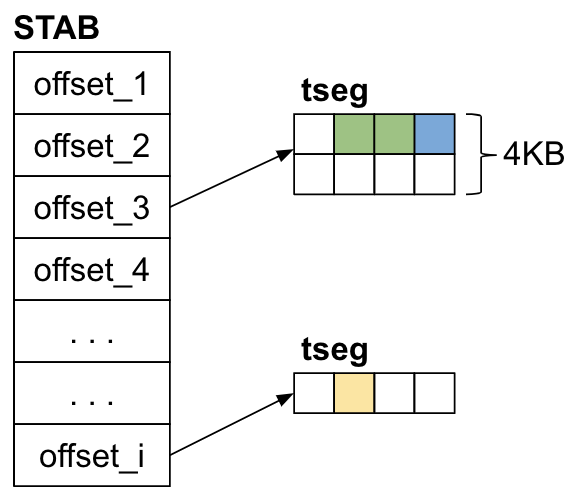
\includegraphics[scale=.7]{images/techn10}
\caption{Structure of libdft \texttt{STAB} data structure when employing byte-size tags.}
\end{figure}

Each \texttt{STAB} entry corresponds to a page-size area\footnote{The usual page size in $32$-bits Windows architecture is $4$KB.} and holds a $32$-bits offset used to access all memory addresses inside that page. The virtual address tag is retrieved into two steps (see listing \ref{lst:virttobyte}):
\begin{enumerate*}[label=\roman*),itemjoin={,\quad}]
\item the $20$ most significant bits of the virtual address serve as index into the mapping table to get the appropriate offset
\item then, adding the virtual address to the offset, it is possible to get the related tag.
\end{enumerate*}
\begin{lstlisting} [language={C++}, label={lst:virttobyte}, caption={Code snippet to retrieve the tag byte of any memory address.}]
/*STAB[vaddr >> 12] contains the specific offset of vaddr.*/
offset = STAB[vaddr >> 12];
/*
* taddr is the memory map address
* containing the respective byte tag.
*/
taddr = vaddr + offset;
\end{lstlisting}
\item When libdft is configured to work with bit-size tags, it stores a bit tag for each memory byte into a flat data structure called \texttt{mem\_bitmap}. Knowing that $3GB$ is the maximum memory which would be allocated for a process, the utmost size of the \texttt{mem\_bitmap} for each process can be $\frac{3072MB}{8B} = 384MB$\footnote{The intuition is that for each $8$ memory bytes, the map contains exactly $1$ byte. Thus, dividing the highest amount of memory we can get for $8$ we get the number of bytes necessary for the \texttt{mem\_bitmap} to work correctly.}.\\

\begin{figure}[h!]
\centering
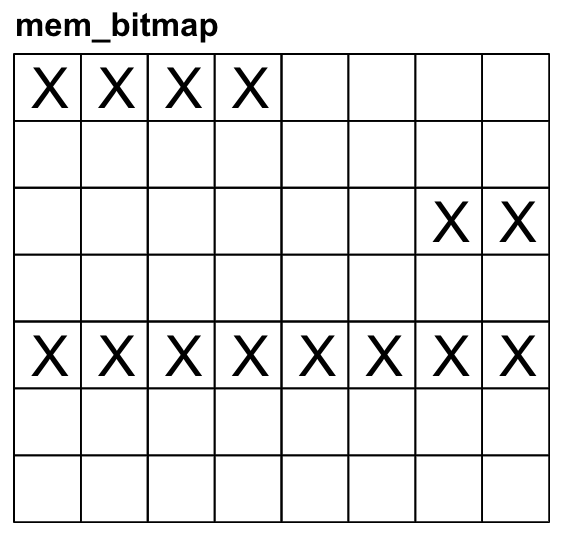
\includegraphics[scale=.6]{images/techn11}
\caption{Structure of libdft \texttt{mem\_bitmap} when employing bit-size tags. Differently from the previous case, here each byte (box-surrounded regions) is either tagged (regions marked with \texttt{x}) or not.}
\end{figure}

When we want to know whether a byte is tainted or not, we need to access this bitmap given the virtual address of the target byte (see listing \ref{lst:virttobit}):. In particular, 
\begin{enumerate*}[label=\roman*),itemjoin={,\quad}]
\item the $29$ most significant bits of the address are used to look for the byte containing tags associated to the virtual address
\item then, the $3$ least significant bits act as offset within the byte retrieved previously.
\end{enumerate*}
\begin{lstlisting} [language={C++}, label={lst:virttobit}, caption={Code snippet to retrieve the tag bit of any memory address.}]
/*
* mem_bitmap[vaddr >> 3] gives the index to get
* the byte associated to vaddr in the mem_bitmap.
*/
idx = mem_bitmap[vaddr >> 3];
/*
* (vaddr & 0x7) gets the three least significant bits of vaddr
* used as offset within the previously obtained byte.
*/
offset = vaddr & 0x7;
/*
* When MASK = 0x1 it allows to obtain the tag bit for a single
* byte. By changing its value, it allows to get the tag bit for
* a word (MASK = 0x3) or even a double word (MASK = 0xF).*/
tval = idx & (MASK << offset);
\end{lstlisting}
\end{itemize}

\subsubsection{Registers Map}
In any operating system, each thread has its own set of registers which is saved and restored any time it, respectively, yields or enters the CPU. Consequently, the tagmap contains a registers map named \texttt{vcpu} for each thread of execution spawned by the process. libdft tracks both thread creation to allocate the \texttt{vcpu} data structure and thread termination to dismantle the virtual CPU.\\
Not all registers are included in the data structure but only general purpose registers (GPR) of the x$86$ architecture are effectively monitored by the library. \\

\begin{figure}[h!]
\centering
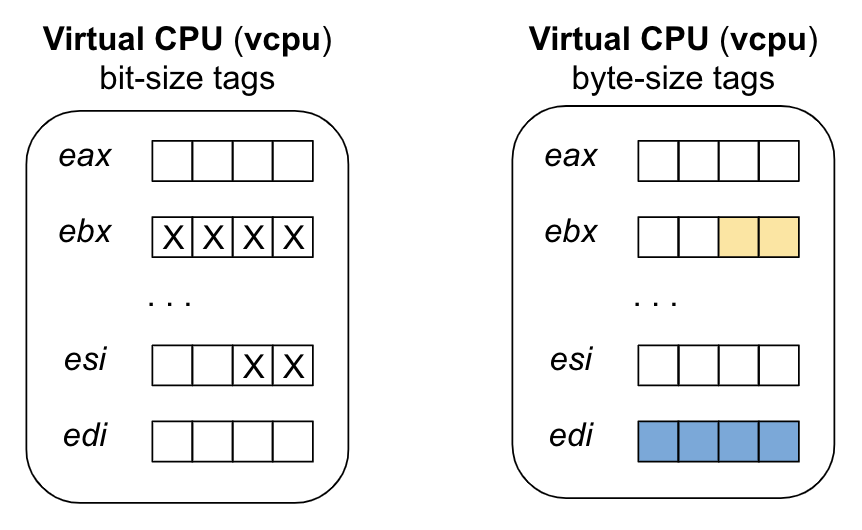
\includegraphics[scale=.6]{images/techn12}
\caption{Structure of libdft \texttt{vcpu} data structure both when using bit-size tags (on the left) and byte-size tags (on the right).}
\end{figure}

\begin{itemize}
\item If the configuration uses bit-size tags, each $32$-bits GPR is represented with $1$ byte in the virtual CPU for a total of $8$ bytes per-thread;
\item When byte-size tags are used, for each $32$-bits GPR, $4$ bytes are required in the virtual CPU up to having $32$ bytes per \texttt{vpcu} data structure.
\end{itemize}
Each virtual CPU is kept inside a liner data structure\footnote{A data structure containing homogeneous elements is said to be linear, if elements stored within the it are organized into a sequence\footnote{li1998linear}.} accessed using an incremental identifier assigned to each thread by Pin.

\subsubsection{Tracker}
\label{subsubsec:taintpropagationlogic}
The module which has the duty of instrumenting the program and injecting analysis functions, is called \textit{tracker}. The steps followed by the tracker to determine which is the appropriate analysis function to insert are the following:
\begin{enumerate}
\item Identify the instruction type. libdft handles four different instruction categories: those performing arithmetic operations, instructions which move data, those untagging the operands and, in the end, instructions which need a special handler;
\item Determine the type (e.g., register, memory) and the length of each operand;
\item Combining these information to decide which is the suitable analysis routine to inject.
\end{enumerate}
An analysis routine is the core component in libdft because it is the element which carries out the dynamic flow tracking logic for each single instruction. Moreover, being executed at each instruction, it is of primary importance that analysis functions introduce the slight overhead possible. Given the features offered by Intel Pin and observations made on the number of inlined instructions by the framework, the authors tuned analysis routines so that: updates of the tagmap are done with a single assignment and no branch is used in analysis functions.\\

libdft offers four different set of analysis functions, each one based on the tracked instruction type. Besides, each set is internally divided depending on whether the library is configured to use bit-size or byte-size tags and according to the size of each instruction operand. When byte-size tags are used and input operands are tagged with different colours, depending on the operation, libdft provides a policy for combining the input tags (constants operands are always considered untagged).

\begin{figure}[h!]
\centering
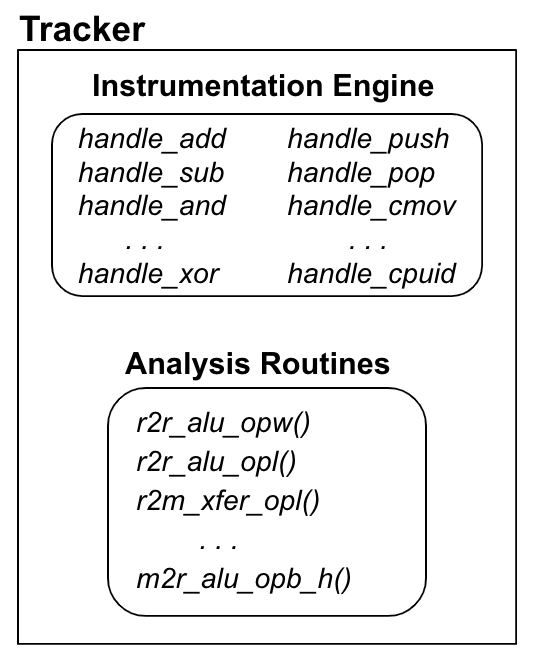
\includegraphics[scale=.6]{images/techn13}
\caption{The \textit{tracker} is the module in charge of instrument the binary (through the \textit{instrumentation engine}) and injecting \textit{analysis routines}.}
\end{figure}

The four different instruction categories which are tracked by the library, are the following:
\begin{itemize}
\item Instructions performing arithmetic operations like \texttt{add}, \texttt{and} and \texttt{sub}. For this category, the destination operand(s) tag is the \textit{union} between the tag of source and destination operands;
\item Instructions transferring data between their operands. In this class are included data movement between register and memory, between two registers and also between memory operands. In this case, the policy is straightforward because the source tags are simply copied into the destination tags;
\item Instructions that cause operands tags to be cleared;
\item Instructions which are regarded as special because cannot be handled by analysis function which fall in the previous classes.
\end{itemize}

\subsubsection{I/O Interface}
The \textit{I/O interface} module is in charge of managing data exchanged by the user-space and the kernel through system calls. Indeed, being written for the Linux kernel, this component holds a huge data structure called \texttt{syscall\_desc[]} containing meta-information used by libdft during the execution, for each of $344$ Linux system calls (up to v2.6.39). Specifically, the \texttt{syscall\_desc[]} is a table storing descriptors for call arguments, whether the system call writes or reads data or also possible user-supplied callbacks for using the call as taint source or sink.\\
When a system call is invoked by the process, the two stubs \texttt{pre\_syscall()} and \texttt{post\_syscall()} are called, respectively upon entry and exit. The purpose of these stubs is twofold:
\begin{itemize}
\item They allow the tool to register hooks on specific system calls like those network- or file-related in order to apply tags to data. This features makes possible to define system calls as taint sources (if the hook is registered on-entry) and taint sinks (when hooks are invoked on-exit);
\item The \texttt{post\_syscall()} stub default behaviour, is to untag data returned or written by the system call. This may be useful when inspecting data manipulated by a taint sink and we want to avoid tags leaking outside the system call. Even though this is the default behaviour, the tool may install a callback specifically for tainting output data from the call.
\end{itemize}

Being libdft originally developed for the Linux kernel, a great effort was employed by BluePill authors, to port the library from the Linux OS and making it compliant to Windows 7 OS. In particular, the \textit{I/O interface} module was not included for obvious reason.

\chapter{DTA-Tracker}
\label{ch:dta-tracker}
In the previous chapter we discussed about how dynamic binary instrumentation is employed by BluePill to neutralise evasive behaviours and how libdft, instead, employs it to design a dynamic flow tracking library. DTA-Tracker is a tool which leverages BluePill capabilities and libdft library for profiling the interaction between the executable and data it manipulates.\\

DTA-Tracker consists of two components: 
\begin{itemize}
\item The first one is in charge of collecting necessary data through dynamic analysis;
\item Then, the second component's task consists in carrying out an offline analysis of gathered information.
\end{itemize}
This chapter describes the two aforementioned components together with insight about adopted techniques and implementation details.

\section{Dynamic Analysis Component}
As already mentioned, in the first step the malware is analysed to get information on how it actually uses memory. This analysis cannot be static rather, it must be dynamic in order to have access to runtime information like memory addresses.\\
Nonetheless, as discussed in \autoref{subsec:evasivemalware}, dynamically analysing a malware can be challenging especially when it adopts artifacts tailored for anti-dynamic and anti-sandbox analysis. For this reason, the malware sample is analysed under BluePill which offers neutralization techniques against these evasive behaviours.

\begin{figure}[h!]
\centering
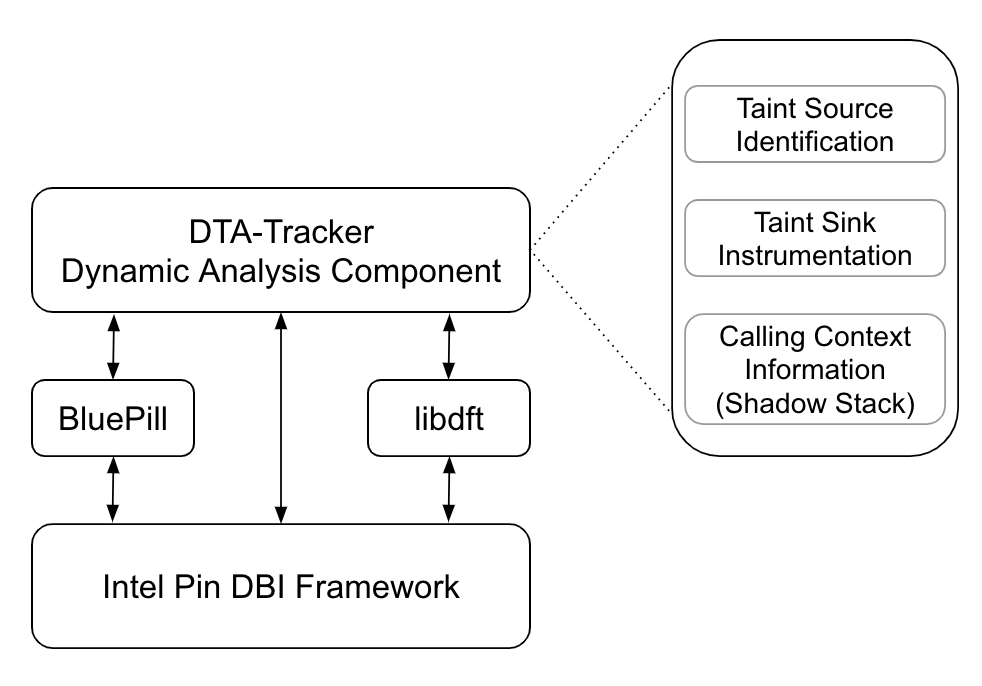
\includegraphics[scale=.6]{images/dtatracker1}
\caption{Bird's eye view of the Dynamic Analysis component of DTA-Tracker.}
\end{figure}
\newpage
\subsection{Identifying Taint Sources}
\label{subsec:identifyingtaintsources}
Before starting any analysis, we need to understand how to choose a source in a way to place taint over it. However, even before, the analyst should be aware of \textit{what} the system considers to be a taint source: DTA-Tracker identifies as taint source, any function and system call which is already hooked in BluePill\footnote{At the moment of writing, DTA-Tracker handles only a subset of the hooks present in Blue Pill, but we have already planned to enlarge this set (see \autoref{ch:futureworks})}.\\

There are many ways to gain the knowledge about which function calls and system calls are leveraged by a malware to carry out its intent, some of which are the following:
\begin{itemize}
\item Looking for reports automatically generated by malware analysis systems (some valid candidates are Joe Sandbox and Hybrid Analysis);
\item Use any static analysis tool (like IDA, pestudio) to extrapolate useful information about imported functions;
\item Take advantage of automatic dynamic analysis tools like BluePill. Indeed, running the malware under this framework, it is possible to get a complete list of function calls and system calls leveraged by the sample. 
\end{itemize}
The behaviour of malicious software can be highly influenced by the environment where it executes. For this reason, the last approach is the most precise because DTA-Tracker will be launched in the same environment where Blue Pill is used.
\begin{lstlisting} [language={TeX}, caption={A subset of function and system calls extracted from a BluePill log file.}]
...
...
[CPUID] - 0x1
[NtQSI-drv] - SystemModuleInformation for system drivers
[NtQSI-proc] - SystemProcessInformation for process check
[NtQSI-proc] - SystemProcessInformation for process check
[NtQueryAttributesFile] - \??\C:\PROGRAM FILES\VMWARE\VMWARE TOOLS
[NtQueryAttributesFile] - \??\C:\PROGRAM FILES (X86)\VMWARE\VMWARE TOOLS
GetAdaptersInfo] - MAC address check
...
...
\end{lstlisting}

\subsection{Tainting Step}
\label{subsec:taintingstep}
When there is a clear vision about the set of function calls and system calls invoked by the malware sample, the next step consists in tainting the output of those calls. However, libdft and consequently also DTA-Tracker, can colour not more than $8$ values at the same time (i.e., during a single execution). This limitation leads to a careful choice of those calls which output shall be tainted. When the number of taint sources is higher than the available number of colours, there are two possible approaches to address the constraint:
\begin{enumerate}
\item Use all the colours to taint more than $8$ output values. In this manner the analyst can surely capture many information at the expense of the quality. Indeed, the details we get from the analysis of a specific tag, do not make possible to trace back to a single taint source but to all taint sources sharing that specific colour;
\item Use one colour to taint only the output of a specific call. In this way, compared to the previous solution, more runs are needed to get the same amount of information. Despite that, even though the quantity of information may be smaller, its quality is for sure better.
\end{enumerate}
For enabling BluePill to start the dynamic taint analysis engine, it must be launched using the \texttt{-taint} option.
\begin{lstlisting}[language=bash]
C:\pin35 > pin.exe -t bluepill.dll -taint -- 
C:\Users\Riccardo\Documents\furtim_sample.exe
\end{lstlisting}
When the option is enabled, a call to \texttt{loadTaintLib()} is performed in order to initialize any data structure required by libdft to work and to switching-on its instrumentation engine. Referring to \autoref{subsubsec:memorymap} and remembering that DTA-Tracker works with byte-size tags, in the initialization step only the segment translation table and the stack shadow memory are allocated by libdft for the process.\\

To give in input the target calls together with the correspondent colours, DTA-Tracker reads a text file named \texttt{colours.txt}. The file structure is quite simple: each line should contain just the hook id and the respective colour separated by a dash. By following this format, the analyst expresses the will to bind a color to the output of a specific call.\\

In order for this procedure to work properly, two constraints must be met:
\begin{enumerate}
\item The first one regards the hook id, which must be a number between $1$ and $255$. Each value between this range, corresponds to a single function or system call except for those which produce a different output (i.e., different data structures) based on the user input (e.g., input flag)\footnote{For example, the system call \texttt{NtQuerySystemInformation()}, produces a different output depending on the value of its second argument.};
\item The second constraint is the colour to be compliant with libdft definition of a colour, that is, any number in the following set: \{\texttt{0x1, 0x2, 0x4, 0x8, 0x10, 0x20, 0x40, 0x80}\}.
\end{enumerate}
Each line read from the file, fills one entry in a global data structure containing the binding. Because a simple array would waste precious memory, an hasmap was implemented where the hook id is the key and the taint seed is the correspondent value.

\subsection{Extracting Calling Context Information}
Being a pintool, Blue Pill has its own instrumentation code used to understand when and where to place specific analysis routines. These analysis routines mostly take the form of hooks on Windows function calls or system call which are, indeed, used by DTA-Tracker as taint sources.\\

In order to enhance the accuracy of information produced by DTA-Tracker, more instrumentation code and more (fine-grained) analysis routines should be added to Blue Pill. Indeed, when introducing the goal of the tool (\autoref{ch:dta-tracker}), we said that we would like to identify slices of a malware around which its main features revolve. However, without the appropriate data structures and without the right management logic, it is possible to to run the risk of being inaccurate.

\subsubsection{Function Detection Using Nucleus\cite{andriesse2017compiler}}
When talking about function detection, the most adopted approach consists in leveraging signature databases. These databases contain function prologues and epilogues of well-known routines, which can be scanned to understand if the binary under analysis matches these patterns. If they match then, with a certain degree of error, it is likely that the function in the binary sample is the same one identified by that signature.

\begin{lstlisting} [language={[x86masm]Assembler}, caption={Example showing a subset of function signatures generated by the tool ByteWeight\cite{bao2014byteweight}.}]
aaa->0.
aad    \$0x0+->0.
aad    \$0x[1-9a-f][0-9a-f]*->0.
aam    \$0x0+->0.
aam    \$0x[1-9a-f][0-9a-f]*->3.40854863999e-05
aam    \$0x[1-9a-f][0-9a-f]*;aad    \$0x[1-9a-f][0-9a-f]*->0.
aam    \$0x[1-9a-f][0-9a-f]*;aam    \$0x[1-9a-f][0-9a-f]*->0.
aam    \$0x[1-9a-f][0-9a-f]*;aas->0.
aam    \$0x[1-9a-f][0-9a-f]*;adc    %ah,%al->0.
aam    \$0x[1-9a-f][0-9a-f]*;adc    %ah,0x[1-9a-f][0-9a-f]*->0.
aam    \$0x[1-9a-f][0-9a-f]*;adc    %al,(%eax)->0.
aam    \$0x[1-9a-f][0-9a-f]*;adc    %bh,%ah->0.
aam    \$0x[1-9a-f][0-9a-f]*;adc    %bh,%al->0.
aam    \$0x[1-9a-f][0-9a-f]*;adc    %bh,(%edx)->0.
aam    \$0x[1-9a-f][0-9a-f]*;adc    %bh,0x[1-9a-f][0-9a-f]*(%ebp)->0.
aam    \$0x[1-9a-f][0-9a-f]*;adc    %ch,-0x[1-9a-f][0-9a-f]*(%eax)->0.
\end{lstlisting}

However signature databases suffer from several disadvantages:
\begin{enumerate}
\item At first, generated signatures are compiler-specific. Depending on the type of compiler (e.g., \texttt{clang}, \texttt{gcc}, \texttt{g++}), function prologues and epilogues vary and so does the signature;
\item While a good level of accuracy can be reached when a binary is not optimized, things get harder when the binary is compiled with an high optimization level;
\item In the end, a signature database can be seen as a blacklist of functions. Hence, as any other blacklist, to be effective it must be continuously updated.
\end{enumerate}
In this context, Nucleus is an open-source, compiler-agnostic, function detection tool. Being compiler-agnostic, the output of the analysis is not influenced by the compiler through which the binary is produced. In order to identify a function in a binary, the tool has to 
\begin{enumerate*}[label=\roman*),itemjoin={,\quad}]
\item locate all addresses denoting a function entry point
\item and then identify the function first and last address.
\end{enumerate*}
Nonetheless, this task is not as easy as it may seem because especially in highly optimized code, there are several challenges to solve including multi-entry and inline functions. Nucleus tries to address all these issues using different heuristics.\\

Thanks to the fact that it is an open-source tool, we had the possibility to access its source code and apply some small changes. In particular, we modified the output file format until having a text file where each line identifies a function whit a pair \texttt{<start\_address>} \texttt{<end\_address>}. The file containing function boundaries generated by Nucleus must be provided to BluePill before actually starting the analysis.\\
When the file is given in input to Blue Pill, DTA-Tracker starts parsing it line-by-line and inserts each interval into an appropriate data structure. The main requirements of this data structure, are two: supporting fast insertion of intervals and efficiency search for the membership interval of any address. According to these two specifications, the choice settled on a binary tree where each node is an interval, namely, a\textit{binary interval tree} data structure.\\ 
The process described above would be an optimal solution under different point of view:
\begin{enumerate}
\item The first one surely regards performances. Since the function boundaries identification is performed statically, it avoids the performance overhead which afflicts any other dynamic approach. Moreover, thanks to the choice of holding intervals into an interval tree data structure, allows to have good performances for both insertion and search operations;
\item The second one is about accuracy. Indeed, thanks to the heuristics adopted by Nucleus it is possible, in principle, to reach an higher accuracy especially when having multi-entry point functions.
\end{enumerate}
Must be pointed out, tough, that results were not as precise as the expectations. Indeed, the function boundaries identified by Nucleus were not just inaccurate rather, most of them were completely wrong.\\

While a binary computer program can have multi-entry functions, it is not possible to find functions overlapping with each other. For several binary files, we noticed that Nucleus produced such wide intervals to incorporate a number of other intervals inside. Besides, the high number of these imprecisions, leads to an incremental loss of accuracy. This is the main reason that led to abandon the idea of adopting Nucleus in DTA-Tracker.\\
Furthermore, there are some limitations inherently static analysis which make it ineffective when applied to certain malware families. For instance, if Nucleus is adopted to identify function boundaries for a packed malware, the reminder part of the analysis would be completely wrong. When the malware unpacks itself, it unveils a completely new binary executable with a different layout. At this point, the information gathered statically, before the execution, would not match those at runtime.

\subsubsection{Shadow Call-Stack}
If it is not possible to find a solution through static analysis, the only remaining way is adopting a dynamic approach. Specifically, instead of relying on a static analysis step to identify function boundaries, the routine are directly recognized during dynamic analysis. This is possible by introducing a new data structure and a completely different approach from the previous one.\\

The \textit{call-stack} is a data structure which allows to know, during the execution of a program, which are the active subroutines at any given time\cite{de2018now}. Therefore, the purpose of the shadow call-stack is different from the one of the real stack data structure maintained by the OS. The only common point between the operating system stack and the call-stack kept by DTA-Tracker, stays in the fact that is per-thread, dynamically allocated at thread creation time and dismantle when the thread terminates. Each of these call-stacks is kept inside a larger data structure which, in turn, is indexed by an id uniquely assigned by Pin at thread creation time.

\begin{lstlisting} [language={C++}, label={lst:shadowstack}, caption={Shadow call-stack related data structures.}]
/*Data structure identifying a single call-stack frame.*/
typedef struct callStackFrame_t {
	/*Target address of call instruction.*/
	ADDRINT calladdr; 
	/*Estimated return address.*/
	ADDRINT retaddr;
	/*Stack pointer value at call time.*/
	ADDRINT spaddr;
	/*Context for the actual frame.*/
	ADDRINT context;
} callStackFrame, *callStackFrameP;

/*Per-thread data structure containing the call-stack.*/
typedef struct callStackThread_t {
	/*The per-thread call-stack.*/
	vector<callStackFrame> *callStack; // Shadow stack
	/*Index to the top frame.*/
	UINT32 callStackTop;
} callStackThread, *callStackThreadP;
\end{lstlisting}

As it is possible to see from the code snippet in \ref{lst:shadowstack}, each subroutine can be identified by a triple plus another value which we are going to discuss later in this section. Each time a new function call or system call is invoked by the program under analysis, a \texttt{callStackFrameP} is created and pushed on top of \texttt{callStack}.\\
DTA-Tracker understands that the application is invoking a function or system call, by using DBI to instrument each \texttt{call} instruction encountered during the program execution. Thanks to the unlimited features offered by Pin, an analysis function is injected right before the execution of the \texttt{call} instruction to push a new entry on the shadow call-stack, storing the following information:
\begin{itemize}
\item The target address corresponding to the entry point of the invoked function or syscall;
\item The value of the stack pointer;
\item The return address to which the routine should return (i.e., the instruction address following the \texttt{call} instruction).
\end{itemize} 
Nonetheless, when inserting a new frame, the call-stack could be in an inconsistent state due to possible optimizations and tricks adopted by the malware. For this reason, before actually pushing the frame, the callback performs some safety checks:
\begin{enumerate}
\item If the stack pointer value of the top call-stack frame and the new frame is the same and both return addresses match, then it is possible that the the malware performed a \textit{tail call}\footnote{When a binary is compiled using an high optimization level, it is possible that the compiler uses a \texttt{jmp} instructions to directly jump to the next routine avoiding the "overhead" introduced by another sequence of \texttt{call}-\texttt{ret} instructions.}. In such case, no frame should be pushed. This technique is so much adopted by malicious code that it is worthwhile to check for this situation;
\item If we are not in the case described by the previous point, what should be checked before pushing the new frame, is the presence of stale frames in the stack (i.e., frames for which the respective subroutines have already returned). For a frame to be stale, it must have an higher stack pointer value with respect to the one of the new frame\footnote{In all OS the stack grows from higher address to smaller ones thus, when a function returns, the stack pointer is increased.}. Therefore, the whole call-stack is inspected to pop every stale frame and, in the end, the new one can be pushed.  
\end{enumerate}
Furthermore, DTA-Tracker instruments every \texttt{ret} instruction with a callback that properly updates the shadow call-stack when a routine terminates. Given the target address (i.e., where the \texttt{ret} is going to fall back) and the stack pointer value at that moment, the analysis routine works on two steps:
\begin{enumerate}
\item It iterates over the call-stack from top to bottom, to find the most recent frame whose return address matches the one of the \texttt{ret} instruction and whose stack pointer matches the current one;
\item If a frame which meets the previous statement exists, then all the frames between the top stack and one just found (included) are deleted. 
\end{enumerate}
Even though handling corner cases described above can result in a slight overhead, not managing them at all may lead to additive inaccuracies which, at the end of the analysis, produce erroneous results.\\

Leveraging the shadow call-stack, DTA-Tracker defines a \textit{context} as the set of frames contained in the call-stack at a specific time. When a new frame is about to be pushed, the correspondent context is computed by xor-ing its return address with the top frame context. The \texttt{context} variable in listing \ref{lst:shadowstack}, is used to assign a unique identifier to each context in order to understand when during the execution, tainted data is introduced (\autoref{subsec:produceridentification}).

\begin{figure}[h!]
\centering
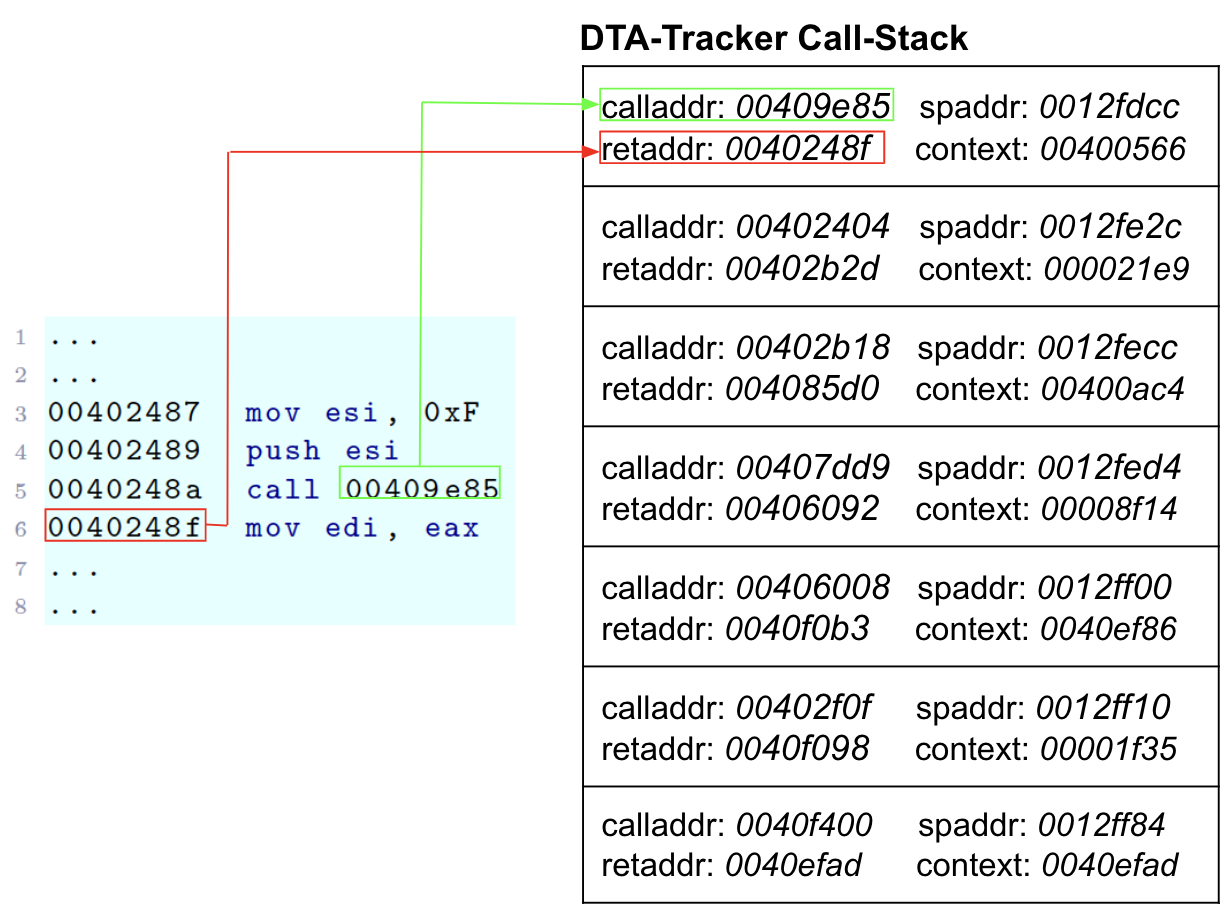
\includegraphics[scale=.5]{images/dtatracker2}
\caption{Graphical representation of a \textit{push} operation on the call-stack.}
\end{figure}
\newpage
\subsection{Identifying Taint Sinks}
\label{subsec:taintsinks}
In the introduction of \autoref{ch:dta-tracker} we already explained that the burden of managing the whole taint propagation logic was left to the libdft library. Thus, having reached this point, what it is missing is the DTA-Tracker, is the definition of taint sink.\\

Information contained inside the shadow call-stack, are necessary to distinguish all the different routines invoked by the malware during its entire execution. As any other computer program, to purse its goal the malware will surely make use of APIs and system calls exported by Windows DLLs, which are consequently tracked and pushed into the shadow call-stack. While the knowledge of APIs and system calls name would be informative, most of the time it is only important know that they "do something" with tainted data.\\
As already mentioned during the discussion above, the ultimate purpose of the DTA-Tracker is to give to the analyst an overview about which malware instructions involve tainted data in their computations. This choice was done for mainly two reasons:
\begin{enumerate}
\item The first one concerns the amount of information produced by the tool. The majority of native APIs and system calls are just stubs that, behind the mask, call different other functions to accomplish their goal. If a malware asks for any OS facility (e.g., API, system call), it is because it will use the output of that request; thus, in case this output contains tainted data, in the end it will be used inside malware routines;
\item The second reason shares similarities with the one above but, at the same time, it is completely different. Keeping track of which native function handles tainted data, would go against the initial objective of the tool, which focuses only on the malware. Indeed, at the end of the day, what a malware analyst wants to know, are which malware routine operate on tainted data and not those from Windows DLLs.
\end{enumerate}
Hence, DTA-Tracker identifies as sinks any movement and comparison instruction which involve tainted data. Most notably, the additional instrumented instructions are:
\begin{itemize}
\item \texttt{mov}. The \texttt{mov} instruction is the most used instructions by compilers to implement data transfer. This feature makes this instruction the perfect candidate to model the malware intent to transfer data either between memory locations and register or also between two memory locations\footnote{Even though the x$86$ instruction set does not provide a \texttt{mov} instruction with two memory operands, it is possible to achieve the same result by concatenating two of them: \texttt{mov reg\_1, mem\_addr\_1}, \texttt{mov mem\_addr\_2, reg\_1}.};
\item \texttt{cmp} \& \texttt{test}. Whilst \texttt{mov} is the most popular instruction (among compilers) to implement data transfer, \texttt{test} and \texttt{cmp} instructions are the most used to implement checks about the content of registers or memory addresses. For this reason, it is fair to imagine that malware checks on tainted data are compiled to one of these two instructions;
\item \texttt{sub}. The point of tracking also the \texttt{sub} instruction, is because even if it is categorized as an arithmetical instruction, it can still be maliciously used to compare two operands. Indeed, as described in the Intel Developer's Manual\cite{intel2018intel}, the \texttt{cmp} comparison is performed by subtracting the second operand from the first one (setting the \texttt{eflags} accordingly).\\
To distinguish the two cases when it is used as a normal arithmetic instruction, from when it is possibly employed to perform comparisons, a little expedient was introduced. Usually, when a computer program checks the value of a specific object, is because the control flow should be altered based precisely on its value. Depending on the result of a comparison, the x$86$ instruction set allows to change the control flow of a program by setting precise flags in the \texttt{eflags} register and using\ textit{conditional jump} instructions. Thus, DTA-Tracker includes \texttt{sub} instructions in the set of tainted sinks only if between that \texttt{sub} and a conditional jump, there is no other \texttt{cmp} or \texttt{test} instruction which can alter the control flow of the program.
\end{itemize}

\subsection{(First) Macro-Phase Output}
All the information gathered from the dynamic analysis are flushed into different files. When writing to a file, better performances can be achieved by implementing a buffering mechanism: instead of directly writing information to the file time by time, a buffer could be used to hold these information up to a fixed size. Once the buffer reaches its limit, it can be flushed into the file.\\
The performance boost from the buffering technique can be significant but it is not always applicable, especially when analysing malware. Indeed, it is not always obvious that a malicious computer program terminates just like any other commodity software. This is the reason why DTA-Tracker flushes data directly to the file whenever new information is available.\\

The first macro-phase produces 4 files, each one containing different information needed in the second phase to produce the final product of DTA-Tracer. The content of each file is the following:
\begin{itemize}
\item \texttt{<exe-name>\_taintedttrace.txt} contains the list of tainted instructions (i.e., taint sinks);
\item \texttt{<exe-name>\_memoryaccesses.txt} contains the mapping between instructions and the tainted memory addresses they have accessed;
\item \texttt{<exe-name>\_contexts.txt} is the file containing the set of unique contexts outlined during the execution;
\item \texttt{<exe-name>\_taintedregions.txt} keeps information about memory addresses tainted in a taint source (i.e., function/syscall hook).
\end{itemize}

\section{Offline component}
At the time when the the files described above are created, the task of the dynamic analysis component is accomplished. Nevertheless, leaving them as they are, is anything but helpful. Indeed, each file contains only a subset of information related to the analysis of the malware, which need to be complemented with all the details contained in the reminder files.\\
One of the major disadvantages of dynamic data flow tracking, is the significant performance overhead introduced by the taint propagation logic: in order to propagate taint, libdft has to carefully inspect each instruction and then inject the appropriate analysis technique. In addition to the instructions instrumented by the library, DTA-Tracker defines its own instrumentation routines which insert analysis functions to fulfill the specific task.\\

Deciding to carry out the analysis whenever new data is available (i.e., on the fly), would degrade performances even more. This is one of the main reasons why DTA-Tracker performs the analysis of gathered information, offline. Hence, the objective of the second macro-phase, is to give a shape to these raw data, producing the final artifact of DTA-Tracker.

\subsection{Producer-Consumer Graph}
It is of fundamental importance that the output of any automatic tool, whether it is static or dynamic, is as explicative as possible. In the same way, a tool which provides detailed information but scattered among different files, would end up being ineffective.\\

The idea we had in mind when designing the final output of DTA-Tracker, was to provide the analyst with fine-grained information maintaining at the same time compactness of data and avoiding the risk of providing scattered results.\\
The \textit{producer-consumer paradigm} imprinted in DTA-Tracker, brings together in a single item, all the elements characterising the taint analysis technique, namely: taint sources, taint sinks and of course, tainted data. The name of this data structure is the \textit{producer-consumer graph} and it is characterized by three building blocks:
\begin{itemize}
\item \textit{Consumers}. A consumer is any malware instruction which involved tainted data in its input operands. We already discussed in \autoref{subsec:taintsinks} what it means for tainted data to be manipulated by a malware routine. Therefore, referring to the nomenclature used in the context of taint analysis, a consumer is nothing but a taint sink;
\item \textit{Producers}. The producer can be seen as the responsible for having caused data to become tainted. Always referring to the taint analysis jargon, in some instances a producer is exactly the source of the tainted flow. Cases in which the producer cannot be identified as the taint source of a flow, are going to be discussed in \autoref{subsec:produceridentification};
\item \textit{Chunks}. Ultimately, a chunk is the memory object "created" by a produced and later manipulated by a consumer (see \autoref{subsec:chunkidentification} for more details). 
\end{itemize}
If consumers, producers and chunks define nodes of the graph, the relationships between nodes are introduced through two different kind of directed edges:
\begin{itemize}
\item The \textit{produces} edge connects the chunk and the consumer: \texttt{chunk\_1} $\rightarrow$ \texttt{consumer\_X}. As the name says, it denotes that \texttt{chunk\_1}  is consumed by \texttt{consumer\_X};
\item The \textit{consumes} edge goes from the producer to the chunk: \texttt{producer\_Y} $\rightarrow$ \texttt{chunk\_1}. It defines that \texttt{chunk\_1} is produced by \texttt{producer\_Y}.
\end{itemize}

\begin{figure}[h!]
\centering
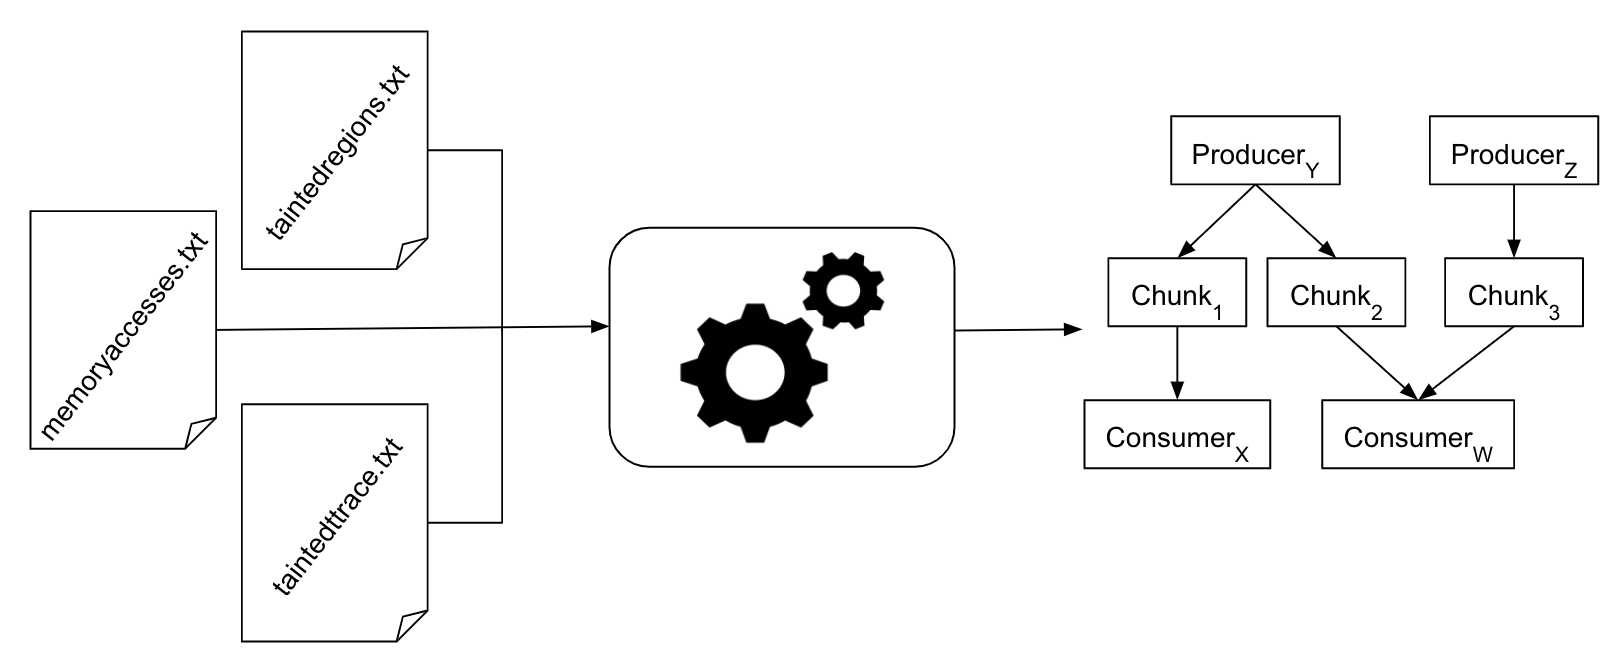
\includegraphics[scale=.45]{images/dtatracker3}
\caption{High level view of the offline component workflow.}
\end{figure}

\subsection{Consumer Driven Approach}
The purpose of DTA-Tracker is to provide an effective and reliable tool which allows the analyst to focus attention on specific portions of the malicious software. According to the original design, the main actors are always malware instructions which manipulate data, that is, the costumers. Hence, for this last reason, the process of building the producer-consumer graph is said to be \textit{consumer-driven}.\\

The first step involves loading the set of consumers identified by the dynamic analysis component of DTA-Tracker during the first macro-phase. Thus, the file \texttt{<exe-name>\_memoryaccesses.txt} is parsed line-by-line to create the list of all consumers as well as the set of all memory addresses accessed (e.g, read, written) by each of them.\\

\begin{figure}[h!]
\centering
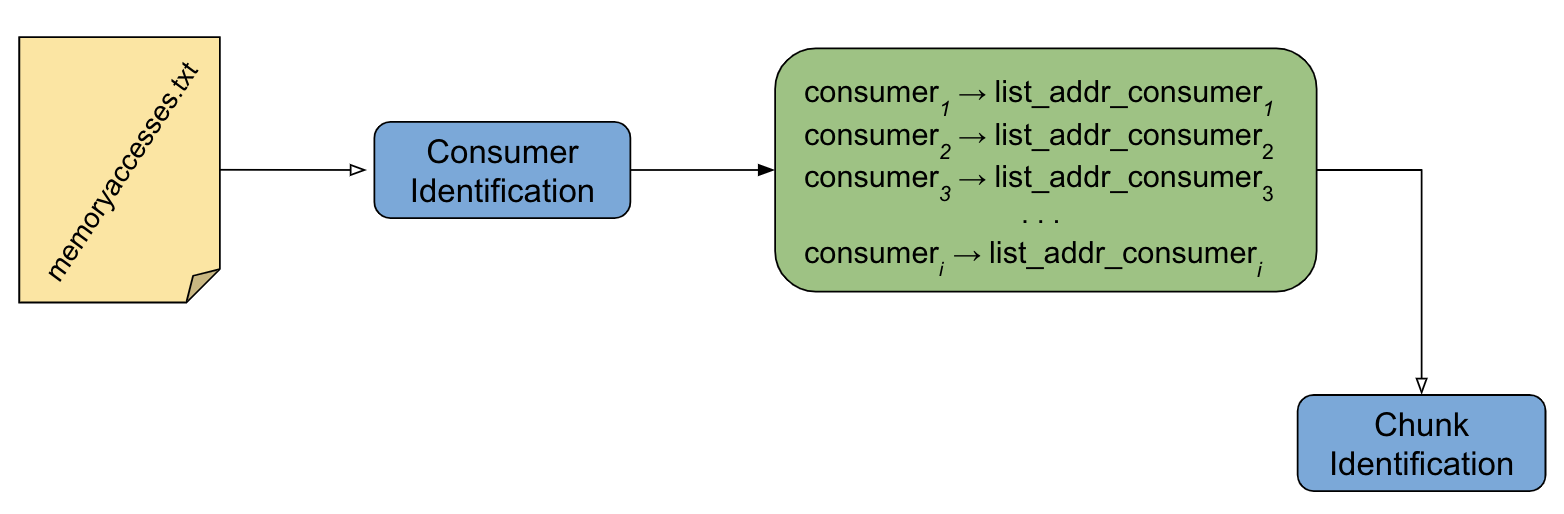
\includegraphics[scale=.6]{images/dtatracker4}
\caption{Consumer identification step where the offline components loads the \texttt{memoryaccesses.txt} file to produce a mapping between consumers and the correspondent list of memory addresses.}
\end{figure}

The consumer node consists in the instruction address which manipulated a chunk of tainted data. However, at this moment, there is no clear idea about the membership chunk of each memory address and in order to define and identify all of them, an additional step is required.
\newpage
\subsection{Chunk Identification}
\label{subsec:chunkidentification}
In the first macro-phase DTA-Tracker records in the memory accesses file, information about instructions which accessed tainted memory addresses. This implies that the dynamic component is aware only of single addresses accessed by the malware. Indeed, at the time when a function accesses a memory location, there is no easy way to understand the memory buffer to which that address belongs to.\\

Therefore, DTA-Tracker defines a \textit{chunk} as a set of adjacent memory addresses which have been used, at least once during the entire program execution, to store tainted data. It is important to notice that during the dynamic analysis of the program, there exist some memory addresses which can be already grouped into chunks. In fact, at the beginning of the analysis, right before the executable is given in input to Blue Pill, it is possible to choose the tainted sources (\autoref{subsec:taintingstep}): whenever the tool faces one of these sources (i.e., function or system call), it will properly taint the output bytes. In the end, these bytes are nothing less than a set of adjacent address that according to the aforementioned definition, correspond to a chunk\footnote{From now on, we are going to refer to these kind of chunks as \textit{type\_1 chunks}.}.\\
While these addresses above are full-fledged chunks, it is also true that they are not the only ones identifiable during the whole program execution. The reason why they are not the only possible chunks, is due to data movement operations. One can think, for example, to a malware routine that just retrieves the data of interest and transfers them to another function which then completes the job. This scenario can, of course, be modeled differently depending both on the compiler and on the optimization level but, in most cases, it will involve more than one chunk.
\newpage
\begin{lstlisting} [language={C++}, label={lst:type2chunks}, caption={Simple example showing how it is possible to cause other memory regions to become tainted, assuming \texttt{ModuleInfo} to be tainted.}]
int aux_func(PRTL_PROCESS_MODULES &ModuleInfo) {
	PVOID ImageBaseArray[1024];
	for(ULONG i=0; i<ModuleInfo->NumberOfModules; i++) {
		ImageBaseArray[i] = ModuleInfo->Modules[i].ImageBase;
	}
	/*
	* do_something with ImageBaseArray[]
	*/
	return 0;
}

int main(int argc, char **argv) {
	PRTL_PROCESS_MODULES ModuleInfo = (PRTL_PROCESS_MODULES)HeapAlloc(GetProcessHeap(), 0, 1024*1024);
	NtQuerySystemInformation((SYSTEM_INFORMATION_CLASS)11, ModuleInfo, 1024*1024, NULL);
	aux_func(ModuleInfo);
	/* . . . */
	return 0;
}

\end{lstlisting}

Hence, one of the tasks of this phase, is to identify chunks\footnote{Chunks constructed in this way are referred to as \textit{type\_2 chunks}.} (e.g, \texttt{ImageBaseArray[]}) resulting from situations like the one in listing \ref{lst:type2chunks}.\\
The technique through which this is possible (called \textit{Fioraldi technique}), requires the data stored into the tainted trace file. Each time that DTA-Tracker finds a tainted instruction, apart from logging information like the instruction type and address, it records:
\begin{enumerate}
\item The memory location accessed by the instruction;
\item Whether the address is used as destination or source operand. This information is particularly important when defining producers (\autoref{subsec:produceridentification};)
\item The amount of bytes read or written by the instruction.
\end{enumerate}
While the tainted trace file is parsed line-by-line, the tool creates a mapping between each memory address and the instructions that accessed it. We use the plural because it is possible to have different instructions accessing the same memory address. Since the trace file contains information about memory locations, through the knowledge of how many bytes were accessed by the instruction, each of them is expanded until having the set of addresses contained in the location.\\

At this point, from a set of addresses, we need to build a set of chunks. The first solution could be grouping a set of contiguous addresses and produce a chunk whose boundaries are the first and the last addresses in the contiguous set. Regrettably, using this method, we risk to create a chunk also including addresses which yet, should belong to a different chunk.\\
To avoid this mistake, the tool keeps track, using an hit counter, of how many times each instruction was encountered while parsing the trace file. Then, the reminder part of the technique consists of the following steps:
\begin{enumerate}
\item Each memory address in the map is associated to the instruction address (in the corresponding instruction set) having the smallest hit counter;
\item Step $1.$ is performed until all memory addresses in the map are associated to one instruction address;
\item In the end, a chunk is created by grouping address sharing the same instruction.
\end{enumerate} 
The last step, can be carried out allowing a \textit{tolerance} factor: a $0$-tolerance factor groups addresses only if they are contiguous while, increasing the factor, makes possible to group addresses which are not necessarily adjacent. Clearly, each choice comes with a trade-off: not allowing any tolerance enables more precision but at the same time, more chunks to manage while a tolerance factor greater than $0$ benefits from managing less chunks resulting in a coarse-grained output.\\

When all the chunks are identified, they can be associated to consumers: from the set of addresses accessed by each consumer, we search for the respective membership chunks, adding a \textit{consumes} edge between chunks and consumers nodes.

\begin{figure}[h!]
\centering
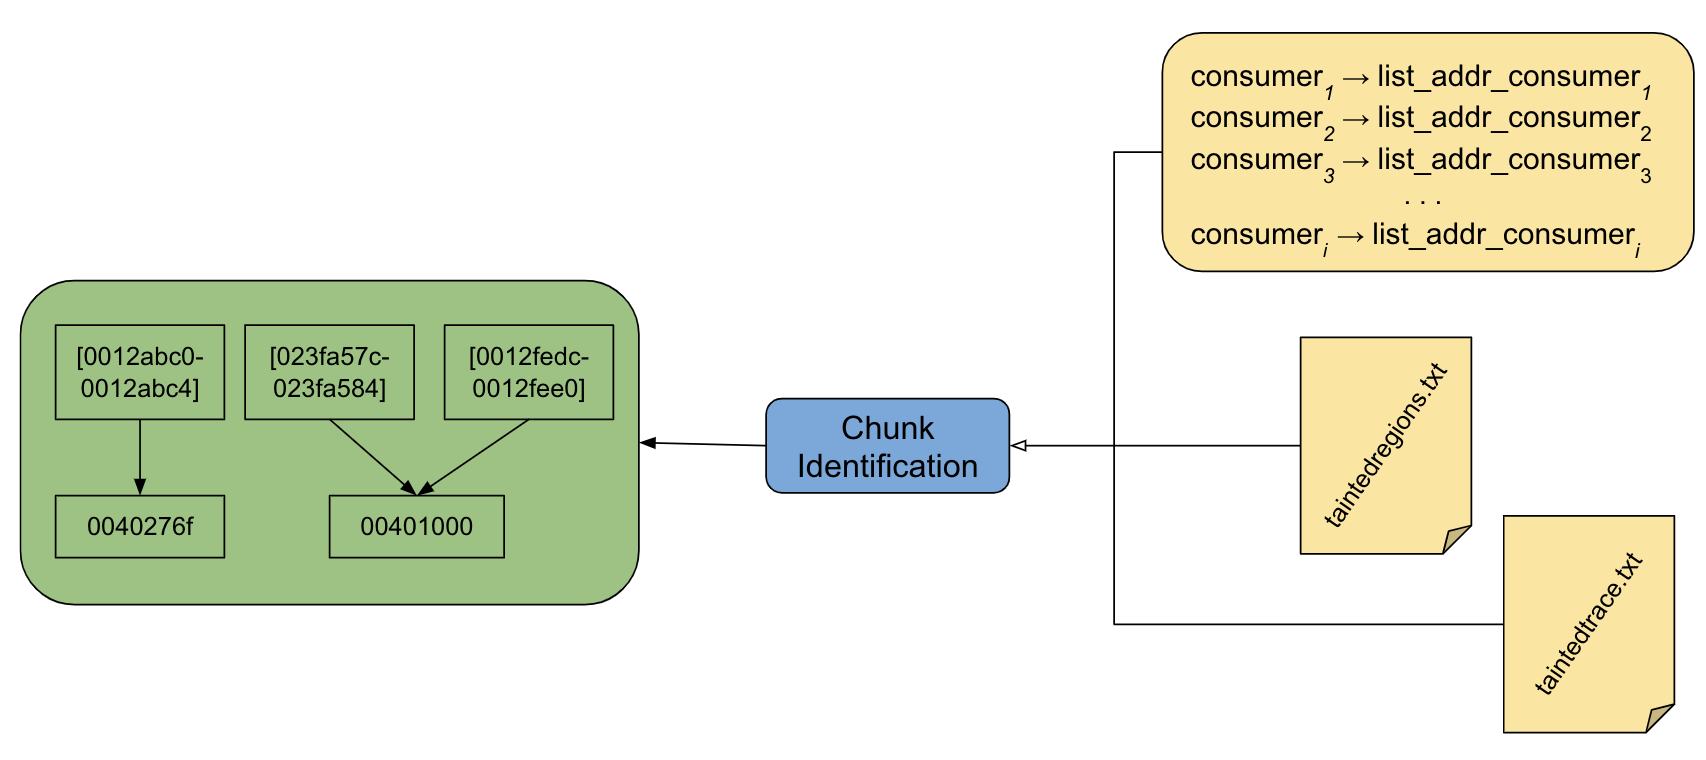
\includegraphics[scale=.5]{images/dtatracker5}
\caption{The offline component loads the two files \texttt{taintedregions.txt} and \texttt{taintedtrace.txt} as well as the output of the consumer identification step, and starts to give a shape to the producer-consumer graph.}
\end{figure}

\subsection{Producer Identification}
\label{subsec:produceridentification}
After identifying type\_1 and type\_2 chunks, the producer-consumer graph contains only the \textit{consumes} relationships. Being a consumer-driven approach, it is natural to focus first on which malware instructions exactly consumed a specific chunk. However, there could not be any consumer without the producer of the chunk. Hence, in order to complete the graph, we need to add also the \textit{produces} relationship between producer and chunks nodes.\\

The producer is defined as the entity responsible for introducing a chunk of tainted data which is later accessed by a malware routine.\\
The first solution that comes into mind, consists in defining a chunk producer as the \textit{allocator} of the memory chunk. There are several ways in which this task can be accomplished but since the tool is implemented through a DBI framework, we decided to instrument functions responsible for memory creation. Specifically, the first instrumented routines were those related to heap management, namely, \texttt{HeapCreate()} and \texttt{HeapDestroy()}. These two user-level APIs are exposed in the \texttt{heapapi.h} Windows header\cite{heapapih77:online} and are used respectively to create and release memory for an heap object. However, by instrumenting these routines, we were not able to reach our goal mainly for two reasons:
\begin{itemize}
\item The first one depends on how Intel Pin works. In particular, when Pin is injected in the input binary, some events, just like the creation of the default heap for the process, are missed. This causes the impossibility to track heap chunks allocated within the default heap;
\item The second reason is that the two APIs are not the only way in which requesting heap creation or destruction. They are only user-level wrapper functions, which internally use Windows low-level runtime routines to carry out the task (i.e., \texttt{RtlCreateHeap()} and \texttt{RtlDestroyHeap()} respectively). Especially in malware, it is possible that low-level functions are used in place of user-level ones as they offer more control over operations.
\end{itemize} 

\begin{lstlisting} [language={C++}, caption={\texttt{RtlCreateHeap()} and \texttt{HeapCreate()} compared, to highlight how the system call can offer more options over heap creation.}]
HANDLE HeapCreate(
  DWORD	flOptions,
  SIZE_T 	dwInitialSize,
  SIZE_T 	dwMaximumSize
);

NTSYSAPI PVOID RtlCreateHeap(
  ULONG              Flags,
  PVOID               HeapBase,
  SIZE_T               ReserveSize,
  SIZE_T               CommitSize,
  PVOID               Lock,
  PRTL_HEAP_PARAMETERS Parameters
);
\end{lstlisting}

In the end, taking into consideration both the aforementioned reasons, we moved our attention to a different set of lower-level calls: \texttt{RtlAllocateHeap()}, \texttt{RtleFreeHeap()} and \texttt{RtlReAllocateHeap()}. The first two functions are declared in the \texttt{Ntifs.h} header\cite{Ntifshhe84:online} file while the last one is undocumented. Deciding to analyse these functions rather than the ones presented above, makes possible to get more precise information about each single heap chunk.\\
Nonetheless, being low-level functions, they are widely used by the OS to allocate and de-allocate heap memory, introducing serious performance overhead. Moreover, and most importantly, a malware can employ a specific routine to allocate heap memory which is later tainted in a different function: in this situation the "allocator" is different from the real producer.

\begin{lstlisting} [language={C++}, caption={Code snippet showing the difference between the "allocator" function and the one that actually causes data to become tainted.}]
PVOID allocator_function(SIZE_T size) {
	PVOID ModuleInfo = RtlAllocateHeap(GetProcessHeap(), 0, size);
	return ModuleInfo;
}

int main() {
	PRTL_PROCESS_MODULES info;
	info = (PRTL_PROCESS_MODULES)allocator_function(1024*1024);
	NtQuerySystemInformation((SYSTEM_INFORMATION_CLASS)11, info, 1024*1024, NULL);
	/* do something with info */
	return 0;
}
\end{lstlisting}

Based on the reasoning above, we decided to define a chunk producer through a completely different approach. DTA-Tracker defines three different type of producers where the first one is identified by the dynamic component and the other two can be inferred only in the offline analysis.\\
Belong to the first category of producers, all the taint sources which are given input to DTA-Tracker by the analyst. Whenever a Blue Pill hook related to a taint source is triggered, DTA-Tracker writes down in the tainted regions file, the name of the hook as well as the set of tainted chunks. This is exactly how the offline component can identify producers of the first type. If a chunk accessed by a consumer, is among these previously tainted by a tainted source, then that source becomes the producer of the chunk. Following this approach, for each chunk in the graph already connected to a consumer, we add a \textit{produces} edge if it was produced by a taint source. This category of producers node are represented with a pair consisting of hook name and context when the tainted chunks were produced.\\

However, it is still possible to have chunks which do not have a \textit{produces} relationship with any producer: it is the case of chunks which were created due to data movement operations. The most reasonable solution would be searching, in the trace file, for the instruction which caused a memory location to be tainted through write operations. Actually, this is what DTA-Tracker does:
\begin{enumerate}
\item It parses the file, searching for instructions which overwrite memory locations. Given the set of x$86$ instructions instrumented by the tool (see \autoref{subsec:taintsinks}), the only one\footnote{We want to remind that DTA-Tracker considers \texttt{sub} instructions exactly like \texttt{cmp}.} which implement this behaviour are \texttt{mov} instructions with a memory location as destination operand;
\item For each such memory address, the tool retrieves the last context where it was overwritten. 
\end{enumerate}
At this point, it is possible to use these information to add the remaining producers to the graph. Specifically, for each memory address from $2.$, if the corresponding membership chunk is connected only to a consumer, then a \textit{produces} edge is added between the chunk and the respective context which acts as producer node in the graph.\\
The heuristic described above, allows to find the majority of producers for chunks left without them. Still, it may happen that even applying this heuristic some chunks remain without a producer. This is the case for chunks whose memory addresses have not been overwritten by a \texttt{mov} rather, by any other x$86$ instruction capable of doing so. The last type of producer introduced to overcome this gap, is the last colour owned by any memory address belonging to the chunk. Thus, for all the chunks left without a producer, a \textit{produces} edge is added between them and the last owned colour.

\begin{figure}[h!]
\centering
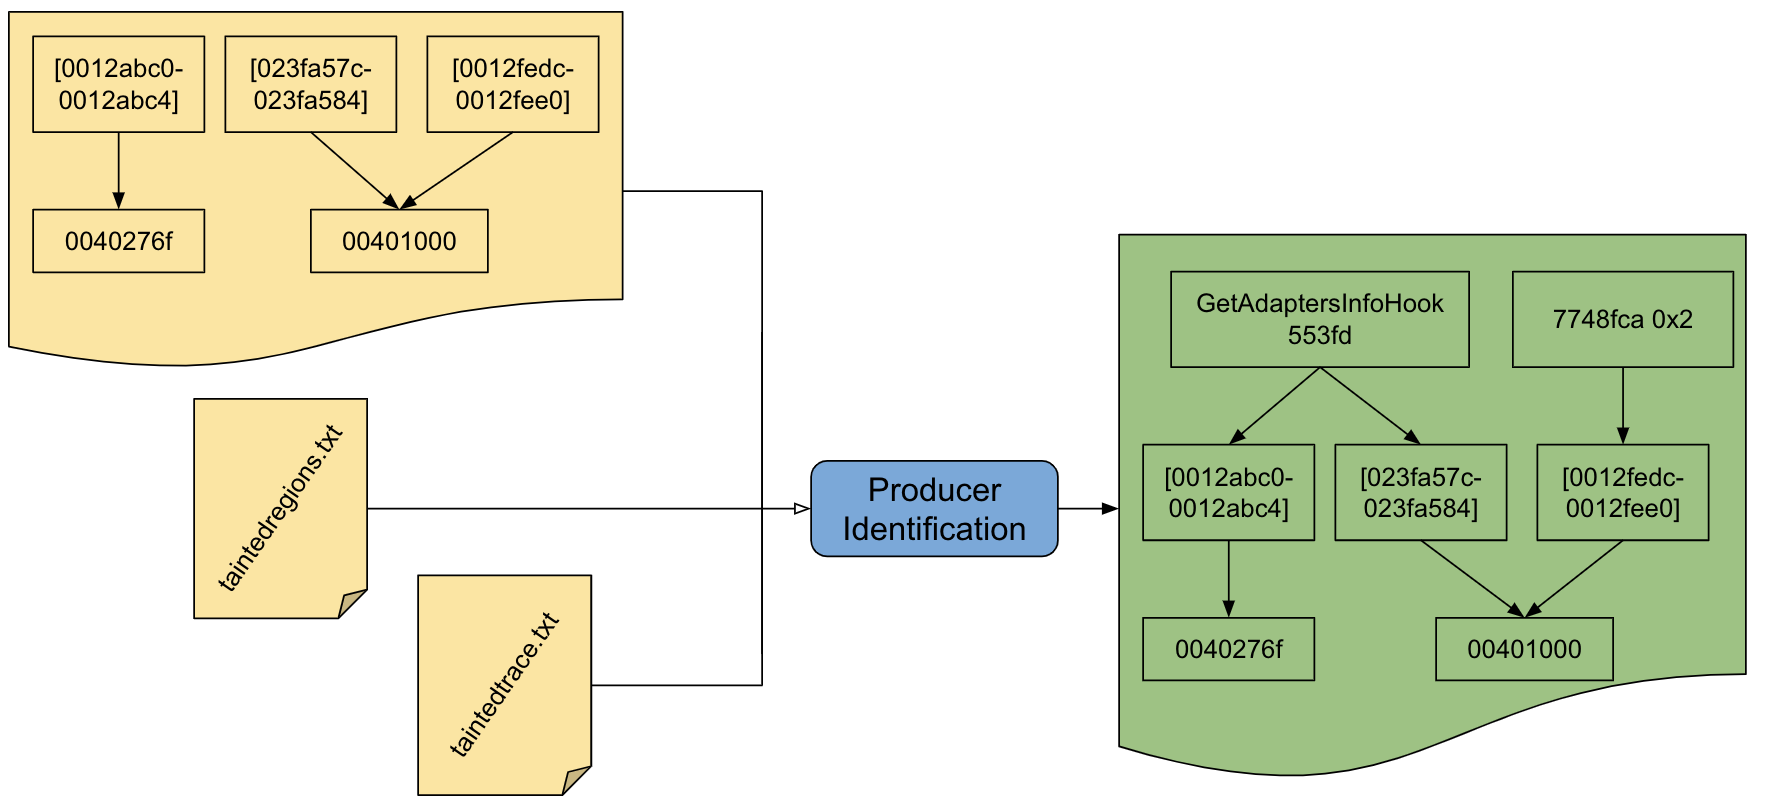
\includegraphics[scale=.45]{images/dtatracker6}
\caption{In the last step, DTA-Tracker identifies all the producers, adding \textit{produce} edges between them and the correspondent chunks.}
\end{figure}

\section{Evaluations/Experimental Results}
\label{sec:evaluations}
DTA-Tracker can be quite helpful as one of the preliminary steps before starting the analysis, allowing the analyst to save time during malware dissection.\\
Being implemented on top of BluePill, we tested the tool on different malicious samples known to expose evasive behaviours. Specifically, the experimental evaluations presented below, are the result of the analysis performed on Furtim\footnote{https://www.sentinelone.com/blog/sfg-furtims-parent/.}, a malware sample known to be highly evasive.

\subsection{Approach}
As explained in \autoref{subsec:identifyingtaintsources}, there are several ways to identify taint sources. For this use-case in particular, we performed a preliminary run of BluePill to discover the set of APIs and system calls leveraged by the sample. At this point, we decided to focus on a subset of these calls assigning to each of them a different colour. There is not any general rule for choosing the set of taint sources nor for assigning them a colour rather, it is up to the analyst who decides what should be tainted. Moreover, depending on the output of the tool, the analyst can decide either to change the set of taint sources or focusing on a specific one, taking advantage of BluePill feature to selectively switch-on and off the countermeasure of each hook.\\
To provide few examples in which DTA-Tracker can be helpful, we chose the following set of taint sources:
\begin{itemize}
\item \texttt{NtQueryAttributesFile} tainted with colour \texttt{0x1};
\item \texttt{cpuid} tainted with colour \texttt{0x2};
\item \texttt{GetAdaptersInfo} tainted with colour \texttt{0x4};
\item \texttt{NtQuerySystemInformation - SystemModuleInformation} tainted with colour \texttt{0x8};
\item \texttt{NtQuerySystemInformation - SystemProcessInformation} tainted with colour \texttt{0x10};
\item \texttt{NtQuerySystemInformation - SystemKernelDebuggerInformation} tainted with colour \texttt{0x20};
\item \texttt{EnumDisplaySettings} tainted with colour \texttt{0x40};
\item \texttt{LoadLibraryW} tainted with colour \texttt{0x80}.
\end{itemize}
\newpage
\subsection{Results}
Running DTA-Tracker with the previously mentioned taint sources and enabling their respective countermeasures, the originated producer-consumer graph is the following:\\

\begin{figure}[h!]
\centering
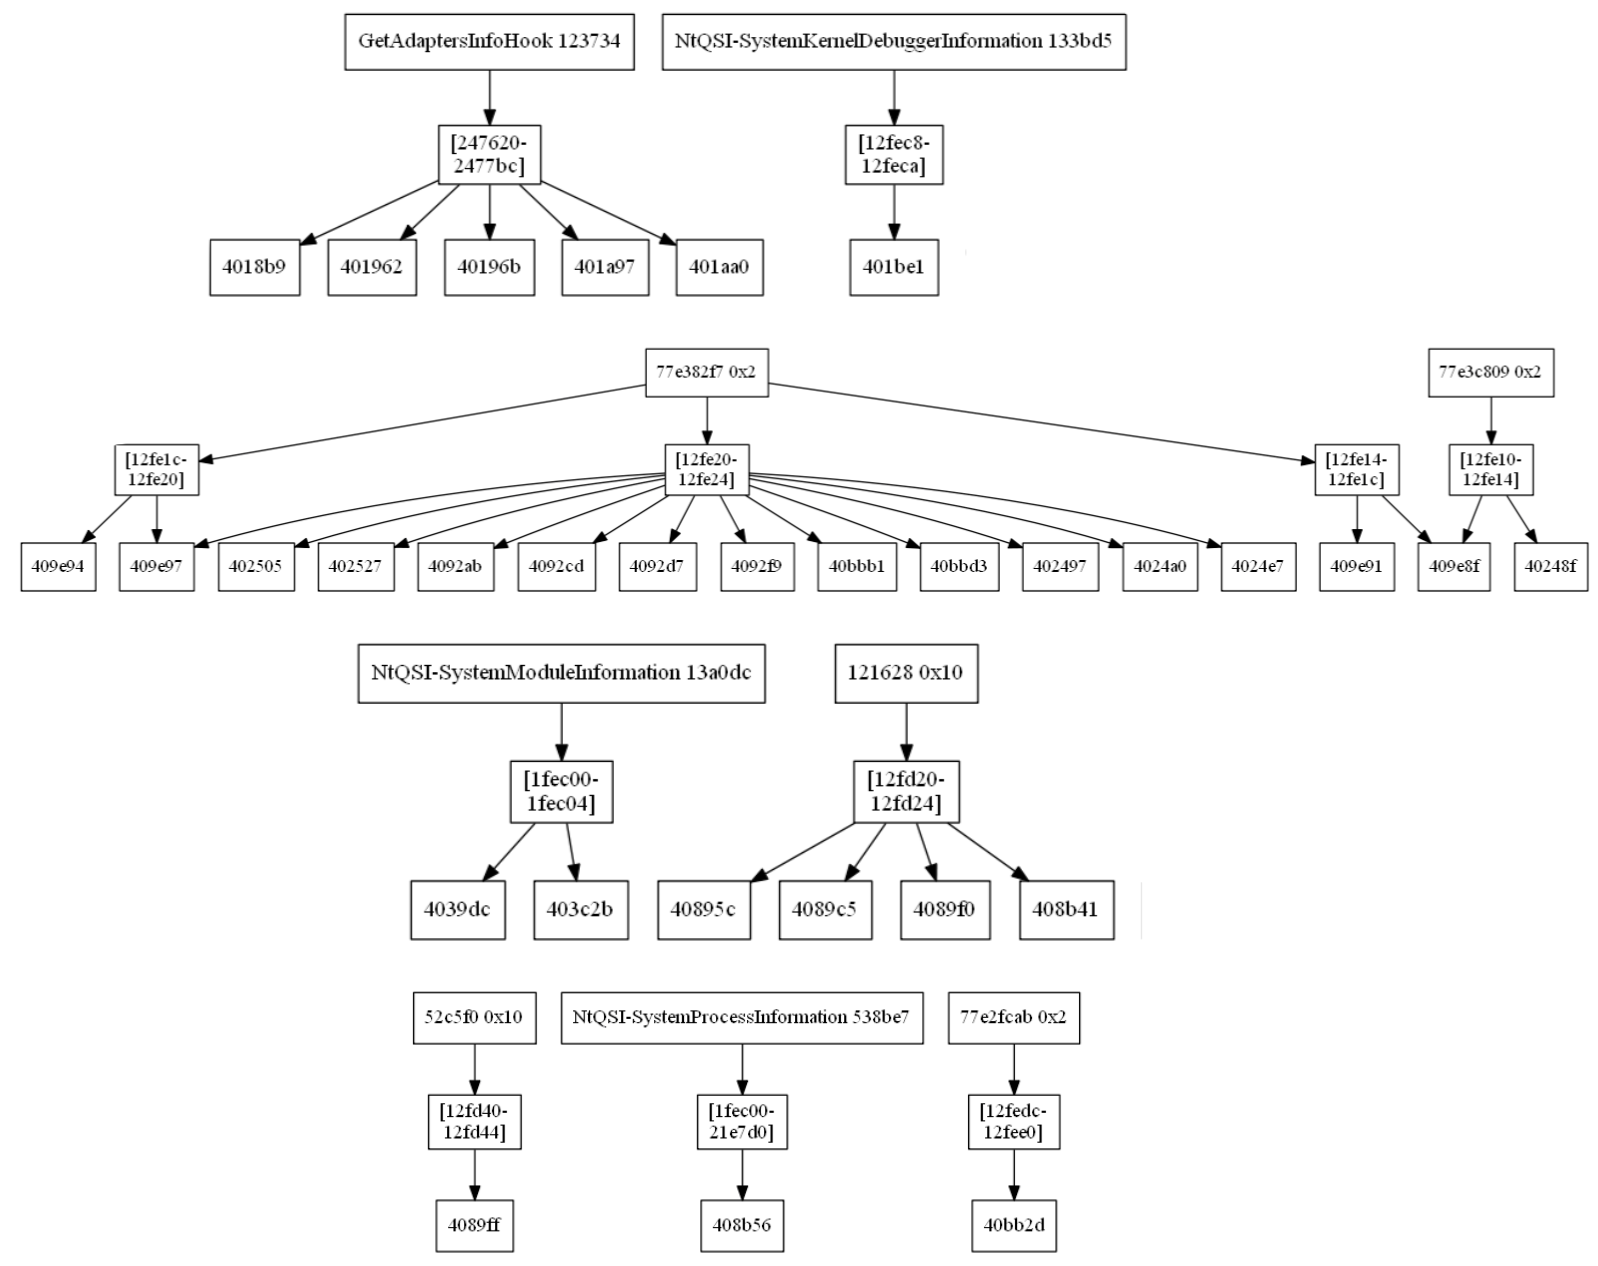
\includegraphics[scale=.5]{images/eval1}
\caption{Producer-consumer graph resulting from a full run on Furtim.}
\label{fig:eval1}
\end{figure}

By looking at the figure, the graph can be divided into three logical levels:
\begin{itemize}
\item The upper level contains the producers;
\item The middle layer is represented by the tainted memory chunks;
\item The lowest level contains the consumers.
\end{itemize}
The producer-consumer graph precisely represents the original goal of DTA-Tracker: provide the analyst with fine-grained information that highlight the interaction (modeled through the producer-consumer paradigm) between sample and data thus, allowing him to save time during dissection.\\
Furthermore, we tried to switch-off different hooks and see whether the producer-consumer scheme could be of any help to the analyst. Specifically, we disabled the countermeasures of two hooks: the first one related to \texttt{NtQuerySystemInformation} with input flag \texttt{SystemProcessInformation} and the other one is the countermeasure of \texttt{GetAdaptersInfo}.\\

The countermeasure present in \texttt{NtQuerySystemInformation} with input flag \texttt{SystemProcessInformation}, hides the presence of running applications which may trigger evasive behaviours. The output of this system call is an array of \texttt{SYSTEM\_PROCESS\_INFORMATION} data structures containing information about each process running in the system. When the respective countermeasure is disabled, the malware can see all the processes names in clear, including those characterising virtualised environments. The result produced by the tool consists in the following graph:

\begin{figure}[h!]
\centering
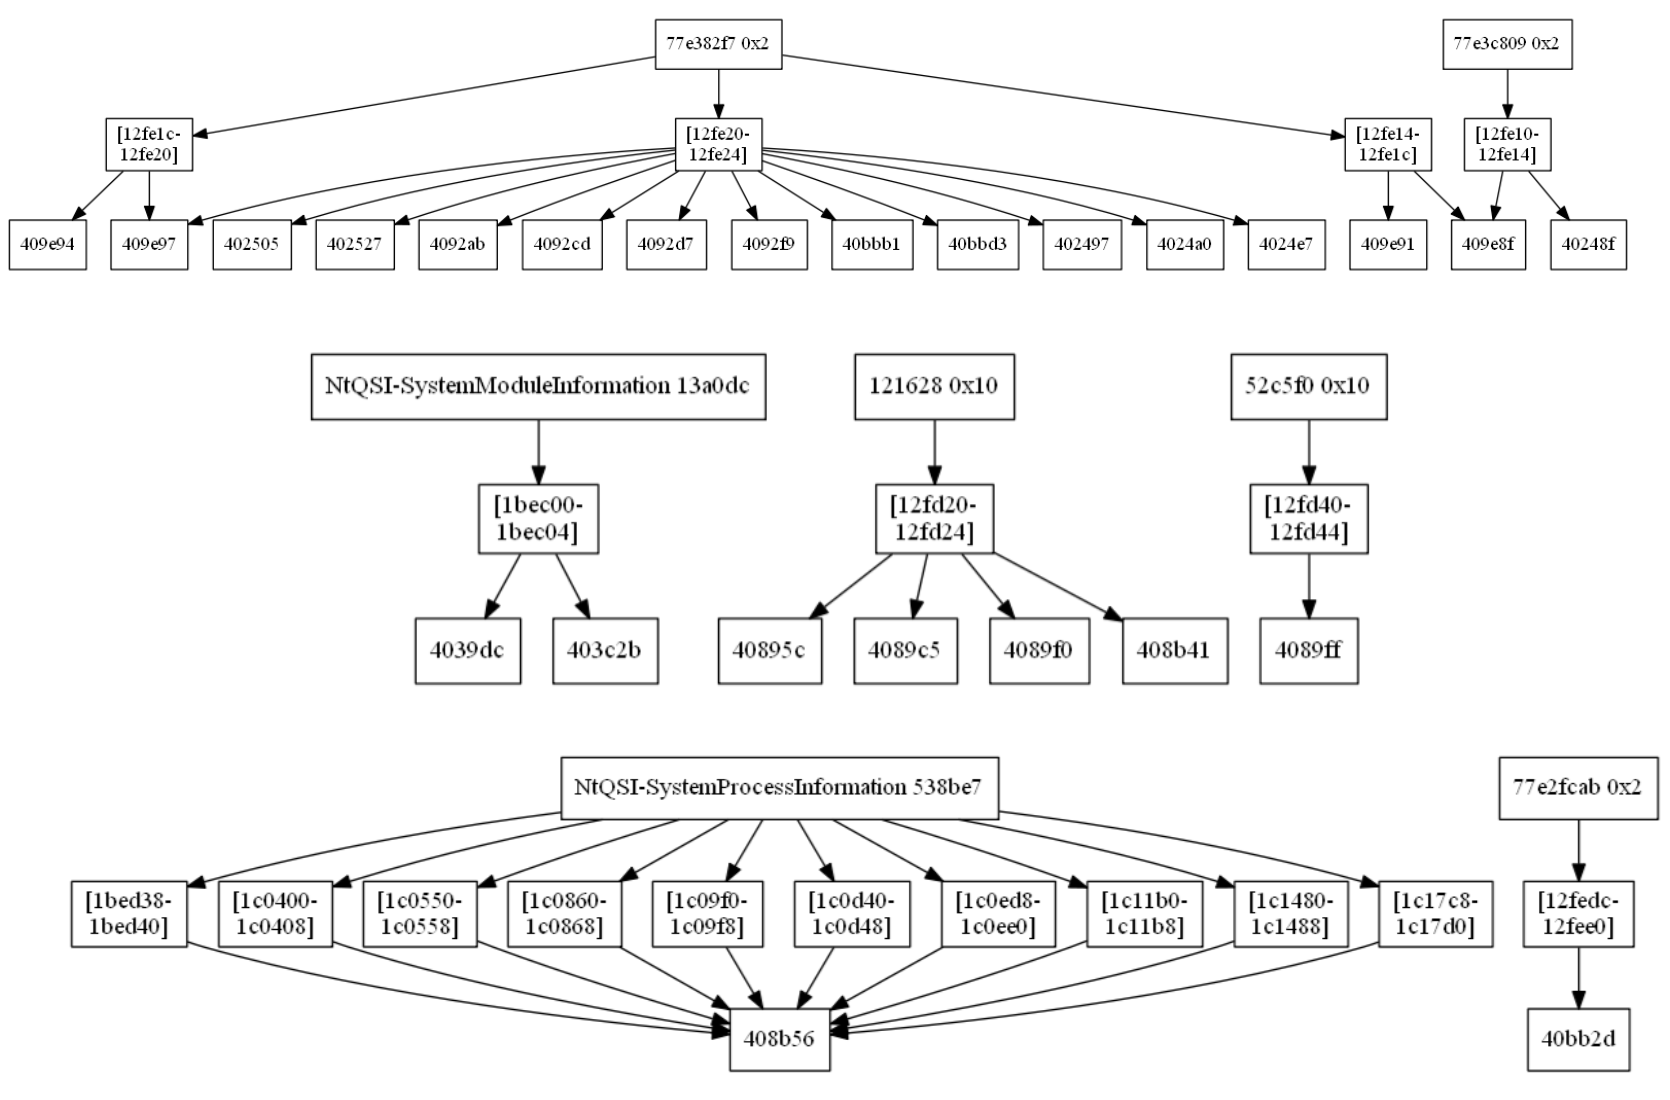
\includegraphics[scale=.5]{images/eval2}
\caption{Producer-consumer graph when Furtim evades due to the lack of \texttt{NtQuerySystemInformation} hook.}
\end{figure}

When a producer creates a number of tainted chunks exceeding a threshold (i.e., 10), DTA-Tracker groups them into a single larger chunk. Although most of the graph is exactly the same as the one in Figure \autoref{fig:eval1}, there is divergence caused by the lack of a countermeasure in the \texttt{NtQuerySystemInformation} hook. Indeed, while in Figure \autoref{fig:eval1} chunks produced by \texttt{NtQSI-SystemProcessInformation 538be7} were grouped into a bigger range because exceeding the threshold, in this case they give precious information for a future dissection. In fact, the graph describes the exact point in the aforementioned array, where the evasion took place.\\ 
Knowing that, the analyst can for example, place a breakpoint close to the instruction identified by the consumer (looking for a possible loop pattern) and step-over as many times as the number of chunks produced by \texttt{NtQSI-SystemProcessInformation 538be7}.\\

Lastly we re-enabled the countermeasure of \texttt{NtQuerySystemInformation} while disabling the one for \texttt{GetAdaptersInfo}. This latter function retrieves information on computer adapters which are often used by malware authors to detect hypervisors and virtual machines. The result produced by DTA-Tracker under these settings, is the following producer-consumer graph:

\begin{figure}[h!]
\centering
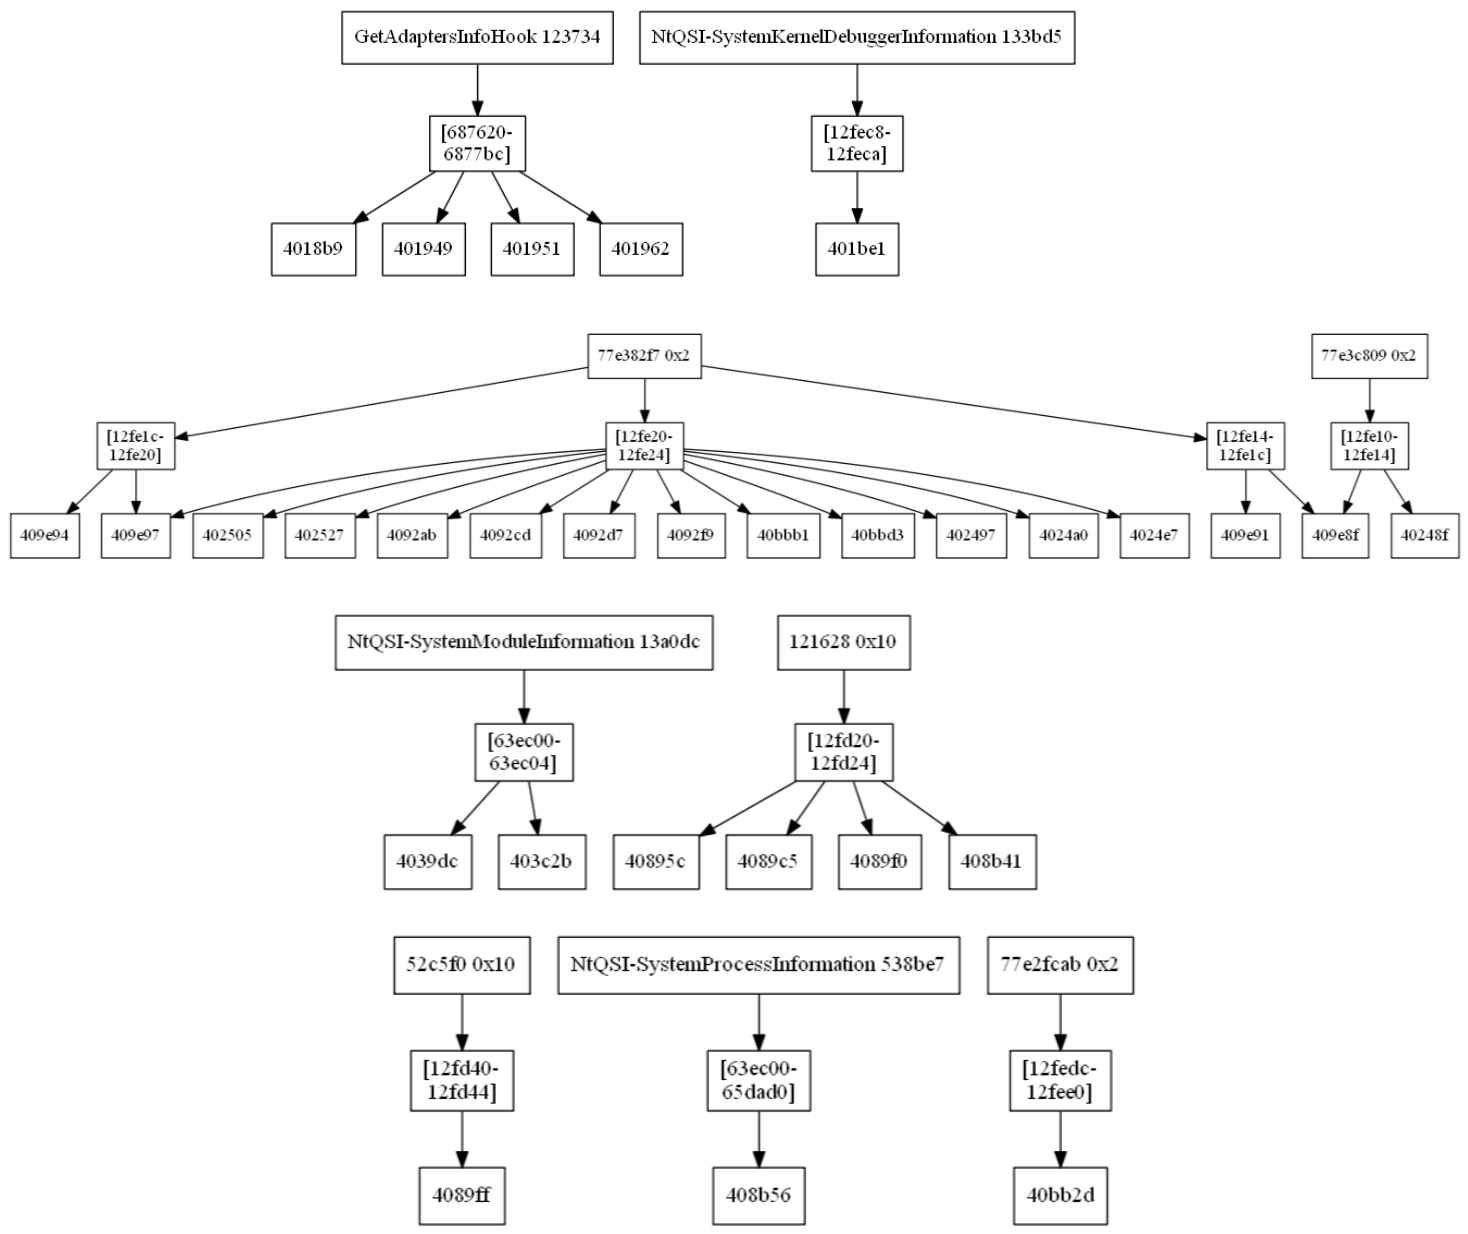
\includegraphics[scale=.5]{images/eval3}
\caption{Producer-consumer graph when Furtim evades due to the lack of \texttt{GetAdaptersInfo} hook.}
\end{figure}

Let us focus on the divergence caused by switching-off the countermeasure in \texttt{GetAdaptersInfo} hook. In particular, it is possible to notice two differences: there are fewer consumers and some of them were not present in the first run. In this case, the analyst can focus on the instruction sequence that lead to the execution of these latter consumers Figure \autoref{fig:eval1} and which is probably the responsible of the premature termination.\\
In fact, we debugged the application following the information provided by DTA-Tracker and we discovered that the two diverging instructions check whether the second and third byte of the network adapter MAC address match with the default ones used in VirtualBox VM (\texttt{00} and \texttt{27} respectively). In this direction, DTA-Tracker is quite useful in situations where the sample presents different instructions sequences depending on different environmental checks.

\chapter{Conclusions and Future Works}
\label{ch:futureworks}
Because of the possibility for a malware to hide implementation details through obfuscation and packaging techniques, static analysis tools are often useless. To remedy this issue, effective automatic dynamic analysis tools and procedures should be used to extract behavioural malware profiles. Nonetheless, several automatic tools fail in unveiling distinctive features of malicious software due to malware authors creativity in devising new methods for slipping through anti-analysis countermeasures. This limitation often forces analysts in resorting to manual intervention from the beginning of analysis. Malware analysts often take a long time to manually dissect binaries, especially due to the lack of a method to identify those slices characterising the executable.\\

We decided to develop DTA-Tracker to avoid inspecting each single instruction of the executable, but providing directions on where to proceed. Leveraging the number of function and system call hooks embedded in BluePill, it makes possible possible to selectively taint the output of different calls. Using a consumer-driven approach, it allows to have a view of program slices where tainted memory is involved in data movement and comparison operations, emphasising the relevant instructions. Moreover, through information collected during the dynamic analysis phase and using reasonable heuristics, the tool provides calling context details about where tainted data originated. Finally, all this knowledge is organized according to a scheme that, as far as we know, had never been applied for this purpose, that is, the producer-consumer graph.



\backmatter
\cleardoublepage
\phantomsection
\addcontentsline{toc}{chapter}{\bibname}
\bibliographystyle{sapthesis} % BibTeX style
\bibliography{bibliography} % BibTeX database without .bib extension

\end{document}